% concatenated from framework-v-main.tex, P101-sur-hom-gadgets-retraction.tex
\documentclass[a4paper,UKenglish,cleveref, autoref,thm-restate]{lipics-v2021}
%This is a template for producing LIPIcs articles. 
%See lipics-v2021-authors-guidelines.pdf for further information.
%for A4 paper format use option "a4paper", for US-letter use option "letterpaper"
%for british hyphenation rules use option "UKenglish", for american hyphenation rules use option "USenglish"
%for section-numbered lemmas etc., use "numberwithinsect"
%for enabling cleveref support, use "cleveref"
%for enabling autoref support, use "autoref"
%for anonymousing the authors (e.g. for double-blind review), add "anonymous"
%for enabling thm-restate support, use "thm-restate"
%for enabling a two-column layout for the author/affilation part (only applicable for > 6 authors), use "authorcolumns"
%for producing a PDF according the PDF/A standard, add "pdfa"

\pdfoutput=1 %uncomment to ensure pdflatex processing (mandatatory e.g. to submit to arXiv)
\hideLIPIcs  %uncomment to remove references to LIPIcs series (logo, DOI, ...), e.g. when preparing a pre-final version to be uploaded to arXiv or another public repository

%\graphicspath{{./graphics/}}%helpful if your graphic files are in another directory

\bibliographystyle{plainurl}% the mandatory bibstyle

\title{Complexity Framework For Forbidden Subgraphs V: Beyond Simple Graphs} %TODO Please add

\titlerunning{Complexity Framework For Forbidden Subgraphs V} %TODO optional, please use if title is longer than one line

\author{Tala Eagling-Vose}{Department of Computer Science, Durham University, UK}{tala.j.eagling-vose@durham.ac.uk}{https://orcid.org/0009-0008-0346-7032}{}

\author{Barnaby Martin}{Department of Computer Science, Durham University, UK}{barnaby.d.martin@durham.ac.uk}{https://orcid.org/0000-0002-4642-8614}{}


\author{Daniel Paulusma}{Department of Computer Science, Durham University, UK}{daniel.paulusma@durham.ac.uk}{https://orcid.org/0000-0001-5945-9287}{}


\author{Siani Smith}{Department of Computer Science, Loughborough University, UK}{siani.smith@lboro.ac.uk}{https://orcid.org/0000-0003-0797-0512}{}

%\author{Tala Eagling-Vose\inst{1}\orcidID{0009-0008-0346-7032} \and
%Barnaby Martin\inst{1}\orcidID{0000-0002-4642-8614} \and
%Dani\"el Paulusma\inst{1}\orcidID{0000-0001-5945-9287} %\and 
%Siani Smith \inst{2}\orcidID{0000-0003-0797-0512
%}
%}

%\authorrunning{T. Eagling-Vose, B. Martin, D. Paulusma, S. Smith}

%\institute{Durham University, Durham, United Kingdom \email{\{tala.j.eagling-vose,barnaby.d.martin,daniel.paulusma\}@durham.ac.uk} \and
%Loughborough University, Loughborough, United Kingdom
%\email{siani.smith@lboro.ac.uk}
%}

%\author{Jane {Open Access}}{Dummy University Computing Laboratory, [optional: Address], Country \and My second affiliation, Country \and \url{http://www.myhomepage.edu} }{johnqpublic@dummyuni.org}{https://orcid.org/0000-0002-1825-0097}{(Optional) author-specific funding acknowledgements}%TODO mandatory, please use full name; only 1 author per \author macro; first two parameters are mandatory, other parameters can be empty. Please provide at least the name of the affiliation and the country. The full address is optional. Use additional curly braces to indicate the correct name splitting when the last name consists of multiple name parts.

%\author{Joan R. Public\footnote{Optional footnote, e.g. to mark corresponding author}}{Department of Informatics, Dummy College, [optional: Address], Country}{joanrpublic@dummycollege.org}{[orcid]}{[funding]}

\authorrunning{T. Eagling-Vose, B. Martin, D. Paulusma, S. Smith} %TODO mandatory. First: Use abbreviated first/middle names. Second (only in severe cases): Use first author plus 'et al.'

\Copyright{Jane Open Access and Joan R. Public} %TODO mandatory, please use full first names. LIPIcs license is "CC-BY";  http://creativecommons.org/licenses/by/3.0/

\ccsdesc[500]{Mathematics of computing~Graph theory}
\ccsdesc[500]{Theory of computation~Graph algorithms analysis}
\ccsdesc[500]{Theory of computation~Problems, reductions and completeness}

\keywords{graph theory, forbidden subgraph, complexity dichotomy, surjective homomorphisms}

%\keywords{Dummy keyword} %TODO mandatory; please add comma-separated list of keywords

\category{} %optional, e.g. invited paper

\relatedversion{} %optional, e.g. full version hosted on arXiv, HAL, or other respository/website
%\relatedversiondetails[linktext={opt. text shown instead of the URL}, cite=DBLP:books/mk/GrayR93]{Classification (e.g. Full Version, Extended Version, Previous Version}{URL to related version} %linktext and cite are optional

%\supplement{}%optional, e.g. related research data, source code, ... hosted on a repository like zenodo, figshare, GitHub, ...
%\supplementdetails[linktext={opt. text shown instead of the URL}, cite=DBLP:books/mk/GrayR93, subcategory={Description, Subcategory}, swhid={Software Heritage Identifier}]{General Classification (e.g. Software, Dataset, Model, ...)}{URL to related version} %linktext, cite, and subcategory are optional

%\funding{(Optional) general funding statement \dots}%optional, to capture a funding statement, which applies to all authors. Please enter author specific funding statements as fifth argument of the \author macro.

\acknowledgements{I want to thank \dots}%optional

\nolinenumbers %uncomment to disable line numbering



%Editor-only macros:: begin (do not touch as author)%%%%%%%%%%%%%%%%%%%%%%%%%%%%%%%%%%
\EventEditors{John Q. Open and Joan R. Access}
\EventNoEds{2}
\EventLongTitle{42nd Conference on Very Important Topics (CVIT 2016)}
\EventShortTitle{CVIT 2016}
\EventAcronym{CVIT}
\EventYear{2016}
\EventDate{December 24--27, 2016}
\EventLocation{Little Whinging, United Kingdom}
\EventLogo{}
\SeriesVolume{42}
\ArticleNo{23}
%%%%%%%%%%%%%%%%%%%%%%%%%%%%%%%%%%%%%%%%%%%%%%%%%%%%%%

\usepackage{graphicx} % Required for inserting images
\usepackage{tikz}
\usetikzlibrary{positioning,automata}
\usepackage{amsmath}
\usepackage{amssymb}
%\usepackage{amsthm}
\usepackage{color}
\usepackage{xypic}[all]
\usepackage[colorinlistoftodos]{todonotes}
\usepackage[utf8]{inputenc}
%\usepackage[russian]{babel}

\newcommand{\DP}[1]{\textcolor{red}{#1}}
\newcommand{\SurHom}{\ensuremath{\mathrm{SurHom}}}
\newcommand{\Ret}{\ensuremath{\mathrm{Ret}}}
\renewcommand{\H}{\ensuremath{\mathbb{H}}}
%\newtheorem{proposition}{Proposition}
%\newtheorem{lemma}{Lemma}
%\newtheorem{corollary}{Corollary}
%\newtheorem{theorem}{Theorem}
%\newtheorem{observation}[theorem]{Observation}

%\title{Cut problems on monotone classes over partially reflexive graphs and multigraphs}
\begin{document}

\maketitle             

%\date{January 2025}

%\date{January 2025}


\begin{abstract}
    We continue the study of the recently-introduced C123-framework, for (simple) graph problems restricted to inputs specified by the forbidding of some finite set of subgraphs, to more general graph problems possibly involving multiedges and self-loops. We study specifically the problems {\sc Multigraph Matching Cut}, {\sc Multigraph $d$-Cut} and {\sc Partially Reflexive Stable Cut} in this connection. The last may be seen as a Surjective Homomorphism problem to a path $P_3$ in which both leaves are looped while the interior vertex is loopless. We consider also another family of Surjective Homomorphism problems to a cycle in which only one vertex is loopless.
    
    When one forbids a single (simple) subgraph, our first three problems exhibit the same complexity behaviour as C123-problems, but on finite sets of forbidden subgraphs, the classification appears more complex. While {\sc Multigraph Matching Cut} and {\sc Multigraph $d$-Cut} have the same classification as C123-problems, already {\sc Partially Reflexive Stable Cut} fails to have. This is witnessed by forbidding as subgraphs both $C_3$ and $H_1$ (which puts {\sc Partially Reflexive Stable Cut} in P). Indeed, the difference of behaviour occurs only around pendant subdivisions of nets and pendant subdivisions of $H_1$. We examine this area in close detail.

    Our other Surjective Homomorphism, ostensibly somewhat similar to {\sc Partially Reflexive Stable Cut}, behaves very differently when the input is restricted to some class that is $H$-subgraph-free. For example, it is solvable in polynomial time on any class of bounded degree. Also, its hardness will never be preserved under any form of edge subdivision.
\end{abstract}

\section{Introduction}\label{s-intro}

In this article, we consider cut problems and their variants. 
%{\sc Matching Cut} and {\sc Stable Cut} 
%(together with a generalisation of the former, called {\sc $d$-Cut}~\cite{GS21} and a variant of the latter). 
{\sc Matching Cut} asks 
for a {\it matching cut}, i.e., an edge cutset that is a matching (so, each vertex has at most one neighbour on the other side of the cut),  while {\sc Stable Cut} asks for a
{\it stable cut}, i.e., a vertex cutset that is a stable (independent) set. 
It is readily seen that a connected graph with no vertex of degree~$1$ has a matching cut if and only if its line graph has a stable cut. 
{\sc Matching Cut}, and thus also {\sc Stable Cut}, is well known to be
NP-complete~\cite{Chvatal1984}.
For $d\geq 1$, {\sc $d$-Cut} asks for an edge cutset
such that
%that the cutset be a union of edges such that each vertex is contained in at most $d$ edges (i.e.,
each vertex has at most $d$ neighbours on the other side of the cut.  Thus, {\sc Matching Cut} and {\sc $1$-cut} are the same.
%equivalent, but we treat {\sc $d$-Cut} as a generalisation of {\sc Matching Cut} since the latter is far better known.

A \emph{homomorphism} from $G$ to $H$ is a function $h:V(G)\rightarrow V(H)$ so that, for all $(x,y) \in E(G)$, we have $((h(x),h(y)) \in E(H)$. A homomorphism is \emph{surjective} if $h$ is a surjective function. Note that this definition also makes sense for graphs with loops permitted. The problem  {\sc Partially Reflexive Stable Cut} is exactly the problem to determine if an input graph has a surjective homomorphism to $P_3^{101}$, where $P_3^{101}$ is the path on three vertices in which both leaves are looped and the interior vertex is loopless. Let us term $\SurHom(H)$ to be the problem defined by graph template $H$ which asks if an input graph $G$ has a surjective homomorphism to $H$. Such problems are well-studied in the literature \cite{GolovachPaulusmaSong,MartinP15} (see also the survey \cite{BodirskyKM12}). Among the most famous of these problems is $\SurHom(C^*_4)$ where, $C^*_4$ is the reflexive $4$-cycle. This problem is also known as {\sc Disconnected Cut} (and the complement of {\sc $2K_2$-Partition}) and was prominent in the literature due to its open complexity until it was settled as NP-complete in \cite{MartinP15}\footnote{Note that Narayan Vikas has an independent proof which is unpublished.}. The complexity of $\SurHom(C^*_k)$ is still not settled for $k \in \{5,6\}$, but for all $k \geq 7$ it is known to be NP-complete \cite{Russian}. Suppose we take a reflexive $k$-cycle and make one of the vertices loopless. Let us call this graph $C'_k$. Note that $\SurHom(C'_k)$ is in P when $k\leq 4$ (this is a consequence of the polynomial algorithm for the retraction problem, as appears \mbox{e.g.} in \cite{Pseudoforests}). It seems $\SurHom(C'_k)$ might behave in a fashion somewhat between $\SurHom(C^*_k)$ and $\SurHom(P_3^{101})$; but it has hitherto not been studied in the literature. We remedy this situation by proving $\SurHom(C'_k)$ is NP-complete for $k \geq 6$.

We study these problems for {\it monotone} graph classes, i.e., classes of graphs that are closed under vertex and edge deletion. Note that many natural graph classes such as planar graphs or bipartite graphs are monotone. Say, for a family of graphs~${\cal H}$, a graph is {\it ${\cal H}$-subgraph-free} if it contains no graph from ${\cal H}$ as a subgraph. 
The recently introduced C123-framework~\cite{JMOPPSL25} (see also \cite{LozinMPPSSL24,JMPPSL23,BodlaenderJMOPPSL25}) considered ${\cal H}$-subgraph-free graphs for finite families ${\cal H}$ and made explicit various ideas that had been largely implicit in the literature (see e.g.~\cite{AK92,GP14,Ka12}). The idea is that if some graph problem $\Pi$ possesses certain properties, then the complexity of $\Pi$ restricted to the class of ${\cal H}$-subgraph-free graphs, for some finite set of graphs ${\cal H}$, can be completely classified as ``hard'' or ``easy'' according to some overarching theorem (at which we will soon alight).

 A graph is {\it subcubic} if every vertex has degree at most~$3$. For $p\geq 1$, the {\it $p$-subdivision} of an edge $e=uv$ of a graph~$G$ replaces $e$ by a path of $p+1$ edges with endpoints $u$ and~$v$. 
The {\it $p$-subdivision} of a graph~$G$ is the graph obtained from~$G$ after $p$-subdividing each edge.
For a graph class ${\cal G}$ and an integer~$p$, let ${\cal G}^p$ be the class consisting of the $p$-subdivisions of the graphs in ${\cal G}$.
 A graph problem $\Pi$ is ``hard'' {\it under edge subdivision of subcubic graphs} if for every $j \geq 1$ there is an~$\ell \geq j$ such that:
if $\Pi$ is ``hard'' for the class ${\cal G}$ of subcubic graphs, then $\Pi$ is ``hard'' for ${\cal G}^{\ell}$.
We can now say that a graph problem~$\Pi$ has property:\\[-9pt]
\begin{itemize}
\item {C1} if $\Pi$ is ``easy'' for every graph class of bounded tree-width;\\[-12pt]
\item {C2} if $\Pi$ is ``hard'' for subcubic graphs ($K_{1,4}$-subgraph-free graphs, where $K_{1,4}$ is the $5$-vertex star);\\[-12pt]
\item {C3} if $\Pi$ is  ``hard'' under edge subdivision of subcubic graphs;\\[-9pt]
\end{itemize}
We say that $\Pi$ is a C123-problem if it satisfies C1, C2 and C3. Let the set ${\cal S}$  consist of all graphs, in which every connected component is either a path or a subcubic tree with exactly one vertex of degree~$3$.  In \cite{JMOPPSL25},  25 C123-problems were identified, and the following meta-classification was shown:

\begin{theorem}[Theorem 3 in \cite{JMOPPSL25}]\label{t-dicho}
For any \emph{finite} set of graphs ${\cal H}$, a \emph{C123}-problem $\Pi$  is ``easy'' on ${\cal H}$-subgraph-free graphs if ${\cal H}$ contains a graph from ${\cal S}$, or else it is ``hard''.
\end{theorem}
\noindent In general, what constitutes ``easy'' and ``hard'' depends on the context. In \cite{JMOPPSL25}, it is usually P versus NP-complete, though sometimes it is almost linear versus quadratic. In \cite{EVMPS24}, it is sometimes P versus complete for some level in the Polynomial Hierarchy. In this article, it will always be P versus NP-complete; see \cite{Leeuwen25} for a recent survey around the C123-framework.

While several related problems, such as
{\sc Perfect Matching Cut}~\cite{LT22} and {\sc Matching Multicut}~\cite{GJMS24}, are NP-complete on subcubic instances, 
both {\sc Matching Cut} and {\sc Stable Cut} are in P for subcubic graphs~\cite{Chvatal1984,Moshi89}\footnote{We note that \cite{CY02} proves a stronger structural result, that every simple graph with at most $2n-4$ edges has a stable cut.}.
Hence, both problems are not C123-problems when considered on simple graphs, as they violate C2. This also means that
in simple graphs, {\sc Matching Cut} and {\sc Stable Cut} satisfy C3 trivially, and {\sc Matching Cut}, though 
not {\sc Stable Cut}, has appeared in \cite{JMPPSL23} discussing C13-problems (those that satisfy just C1 and~C3). However, neither satisfies a version of C3 where NP-hardness of not necessarily subcubic instances is preserved under edge subdivision. In this case, edge subdivision will eventually make all instances into trivial yes-instances.

 As we will now argue, both {\sc Matching Cut} and {\sc Stable Cut} make sense on slightly richer graph structures, possibly allowing multi-edges or self-loops (we call such graphs {\it multigraphs} or {\it partially reflexive}, respectively). Specifically, we can define {\sc Matching Cut} and {\sc $d$-Cut} on multigraphs and {\sc Stable Cut} on partially reflexive graphs. 

In {\sc Matching Cut} a multi-edge can never be in the cutset, while in {\sc Stable Cut} a looped vertex can never be in the cutset. One may deduce the latter from a definition  that we do not allow looped vertices to be members of a stable set in a partially reflexive graph. A natural way to explain the role of loops in {\sc Stable Cut} comes from considering it in its guise as the surjective homomorphism problem to the path $P_3^{101}$ on three vertices, the middle of which is loopless, while the outer two are looped. A {\it surjective homomorphism} from a graph $G$ to a graph $H$ is a function $f:V(G)\to V(H)$ such that for all $(u,v)\in E(G)$, $(f(u),f(v))$ belongs to $H$, and moreover, for every $x\in V(H)$ there exists a vertex $u\in V(G)$ with $f(u)=x$.  Hence, the surjective homomorphisms of an input graph $G$ to $P_3^{101}$ are precisely the stable cuts, where the cutset is read from the inverse image of the loopless vertex. Thus the stable cut must involve only loopless vertices. This realisation of {\sc Stable Cut} as a surjective homomorphism problem 
appeared in \cite{GolovachPaulusmaSong}. 
%
Note that there are no trivial self-reductions from our problems, on multigraphs or partially reflexive graphs, to simple graphs (e.g., by contracting multiedges). It is instead possible to simulate multiedges by the judicious introduction of cliques and the growing of the vertex set (such an approach is used in \cite{GolovachPaulusmaSong} and will appear later in Proposition~\ref{prop:multi-d-cut-bounded-treewidth}). This destroys the natural structure of the input. Consequently, these more general versions of our problems are perfectly natural in and of themselves.
%
In order to avoid confusion with the problems on simple graphs, we will speak henceforth of {\sc Multigraph Matching Cut}, {\sc Multigraph $d$-Cut} and {\sc Partially Reflexive Stable Cut} to emphasise that we allow the correspondingly enriched structures.
 
The question arises how to judge degree in a multigraph or a partially reflexive graph. From the perspective of the C123-framework, the hardness on subcubic instances is required to produce hardness on $K_{1,4}$-subgraph-free instances, so multi-edges (after they are counted once) should not add to degree and neither should loops. Additionally, the C123-framework only says something about what happens when a finite set of simple graphs is omitted and, for now, let us leave it at that. Let us note that our choices are not arbitrary in order to fit into the C123-framework. Rather, they are what is required for the problems on partially reflexive multigraphs to be studied under the forbidding of simple subgraphs.

%The condition C3 is the most contentious in definition, and we will use it asymmetrically in this work. Specifically, we will only subdivide multiedges in {\sc Multigraph Matching Cut} and edges $(u,v)$ in {\sc Partially Reflexive Stable Cut} one of whose ends is a loop, and all the new introduced vertices are looped. In this sense, we will not be able to claim our problems are true C123-problems. However, our method will be enough to garner some classifications.
 
Our work begins by making the relatively straightforward observations that {\sc Multigraph Matching Cut}, {\sc Multigraph $d$-Cut} and {\sc Partially Reflexive Stable Cut} are NP-complete on subcubic instances (for all $d\geq 1$). The question then arises, as to whether they are C123-problems. We prove that {\sc Multigraph Matching Cut} and {\sc Multigraph $d$-Cut} have the same classification as C123-problems, while {\sc Partially Reflexive Stable Cut} is not a C123-problem, yet has the same complexity as one over $H$-subgraph-free graphs (\mbox{i.e.} when just one subgraph is forbidden). In fact, we do not have an example of the latter behaviour for problems on just simple graphs. In the case of {\sc Partially Reflexive Stable Cut}, we make use a weaker version of C3. We can subdivide edges $(u,v)$ only when one of those vertices is reflexive, and then all the newly introduced vertices are reflexive. Note that our results imply a posteriori that the full C3 condition can not hold.

The behaviour of {\sc Disconnected Cut} on $H$-subgraph-free graphs is not well-understood, though it is clear that it behaves equivalently on irreflexive, partially reflexive and reflexive inputs. The problem is open even in the $K_4$-(subgraph-)free case. We believe it is perfectly possible that {\sc Disconnected Cut} is in P when restricted to $H$-(subgraph-)free graphs for all $H$. However, we are able to prove that $\SurHom(C'_k)$ remains NP-complete for $K_{3}$-(subgraph-)free graphs, while being solvable in polynomial time for any class of bounded degree. {\sc Partially Reflexive Stable Cut} is NP-complete on subcubic graphs and {\sc Disconnected Cut} is in polynomial time for $K_3$-subgraph-free graphs \cite{FleischnerMujuniPaulusmaSzeider}. Thus, we see that $\SurHom(C'_k)$ behaves differently from both. This then is our motivation for studying $\SurHom(C'_k)$, a problem somewhat between {\sc Partially Reflexive Stable Cut} and {\sc Disconnected Cut} (see Table~\ref{tab:2}).

We summarise our results as Theorems~\ref{t-1}--\ref{t-4}, which we prove in Section~\ref{s-1}--\ref{s-new}, respectively (we formulate the case $d=1$ for {\sc Multigraph $d$-Cut}
as a separate theorem for {\sc Multigraph Matching Cut}). For reasons of space, some proofs will be deferred to the appendix.

\begin{theorem}\label{t-1}
    Let ${\cal H}$ be a finite set of simple graphs. Consider {\sc Multigraph Matching Cut} restricted to ${\cal H}$-subgraph-free instances. If ${\cal H}$ contains a graph from ${\cal S}$, then this problem is in P; else it is NP-complete.
    \label{thm:matching-main}
\end{theorem}

\begin{theorem}\label{t-2}
    Let $d\geq 2$ and ${\cal H}$ be a finite set of simple graphs. Consider {\sc Multigraph $d$-Cut} restricted to ${\cal H}$-subgraph-free instances. If ${\cal H}$ contains a graph from ${\cal S}$, then this problem is in P; else it is NP-complete.
    \label{thm:d-main}
\end{theorem}

\begin{theorem}\label{t-3}
    Let $H$ be a simple graph. Consider {\sc Partially Reflexive Stable Cut} restricted to $H$-subgraph-free instances. If $H \in {\cal S}$, then this problem is in P; else it is NP-complete. However, there exists a set ${\cal H}$ of two simple graphs, neither of which is in ${\cal S}$, such that  {\sc Partially Reflexive Stable Cut} on ${\cal H}$-subgraph-free instances is in~P. 
    \label{thm:stable-main}
\end{theorem}

\begin{theorem}\label{t-4}
For every $k\geq 6$, $\SurHom(C'_k)$ is NP-complete even for $K_{3}$-subgraph-free graphs. However, it is in P for any class of graphs of bounded degree.
\end{theorem}

We also give a summary of our results in the form of two tables (Tables~\ref{tab:1} and \ref{tab:2}), some further necessary definitions appear in the preliminaries.
\begin{table}
\begin{center}
\begin{tabular}{|c|c|c|}
\hline
 ${\cal H}$ & {\sc Multigraph Matching/ $d$-Cut} & {\sc Partially Reflexive Stable Cut} \\
\hline  
 $S_{j,k,\ell}$ & P & P \\  
\hline
 $H_i^{j,k,\ell,m}$ & NP-complete & NP-complete \\    
\hline
 $C_i$ & NP-complete & NP-complete \\    
\hline
 $\{kN_{1,1,1},H_1^{1,1,1,1}\}$ & P & NP-complete \\
\hline
 $\{N_{1,1,1},H_1^{1,1,1,\ell}\}$ & P & NP-complete \\
\hline
 $\{C_3,H_1^{2,2,2,1}\}$ & P & NP-complete \\ 
\hline
 $\{C_3,H_1^{2,2,2,2}\}$ & NP-complete & NP-complete \\ 
\hline
\end{tabular}
\end{center}
\caption{Our principal results around {\sc Multigraph Matching/ $d$-Cut} and {\sc Partially Reflexive Stable Cut} for ${\cal H}$-subgraph-free instances (see Section~\ref{s-pre} for further definitions).}
\label{tab:1}
\end{table}

\begin{table}
\begin{center}
\begin{tabular}{|c|c|c|c|}
\hline
 $H$ & {\sc \mbox{Part.} \mbox{Ref.} Stable Cut} & {\sc Disconnected Cut} & $\SurHom(C'_k)$ ($k\geq 6$) \\
\hline  
 $S_{1,4}$ & NP-complete & P & P\\  
\hline
 $K_3$ & NP-complete & P & NP-complete \\    
\hline
\end{tabular}
\end{center}
\caption{Our principal results around {\sc Partially Reflexive Stable Cut}, {\sc Disconnected Cut} and $\SurHom(C'_k)$ for $H$-subgraph-free instances (see Section~\ref{s-pre} for further definitions)}
\label{tab:2}
\end{table}

\section{Preliminaries}\label{s-pre}

\emph{Looped} vertices are reflexive and \emph{loopless} vertices are irreflexive. Call a partially reflexive multigraph \emph{subcubic} if the maximum degree of the irreflexive graph underlying it is three, or equivalently $G$ is $K_{1,4}$-subgraph free. This is significant, as by taking the reduction of Patrignani and Pizzonia \cite{MatchingCut} we can show that {\sc Multigraph Matching Cut} is NP-hard on subcubic graphs (whereas their original result only claims this for maximum degree 4). In \cite{MatchingCut} double-edges increased the degree twice allowing the NP-hardness for maximum degree four graphs to translate to simple graphs.

Let $S_{j,k,\ell}$ indicate the {\it subdivided claw}, which is obtained by identifying the ends of paths of length $j,k,\ell$, respectively. Let $kH$ indicate the disjoint union of $k$ copies of~$H$.
Let $N_{i,j,k}$ be the graph formed by adding pendant paths of length $i$, $j$ and $k$ to the vertices of a triangle. In particular, $N_{1,1,1}$ is the {\it net}.

 Let ${H_{i}}$ be the graph obtained by adding a path of length $i$ between the internal vertices of two vertex-disjoint copies, $x_1-y_1-x_2$ and $x_3-y_2-x_4$, of $P_3$. We define ${H^{j_1, j_2, j_3, j_4}_{i}}$ to be the graph obtained from $H_i$ by subdividing the edge incident to $x_k$ $j_k-1$ times for $1 \leq k \leq 4$. In particular, the case $j_1=j_2=j_3=j_4=1$ corresponds to $H_i$ and we omit the superscript. If $j_1=j_2=j_3=j_4=k$, then we may write $H^k_i$. For example, $H^{2,2,2,2}_1=H^2_1$.

In a graph $G$, let $N(u)$ be the set of vertices adjacent to $u$ in $V(G)$. Call a pair of vertices $u$ and $v$ \emph{twins} if $N(u)=N(v)$. If further we have $E(u,v)$, then $u$ and $v$ are \emph{true twins}.

In this paper, $\mathcal{H}$ always refers to a finite set of graphs.

%SS Added H-graph definition, probably there's a better way to write it.

%DP: I commented this out as we do not seem to need it and we used different notation in Section 1.
%If $\alpha\in \{0,1\}^k$, then $P_\alpha$ is a path on $k$ vertices with the $i$th vertex is loopless iff the $i$th digit in $\alpha$ is $0$. For example, $P_{101}$ is the path on three vertices with end points looped and the middle vertex loopless.

\section{Multigraph Matching Cut}\label{s-1}

The {\sc Matching Cut} problem asks if there exists an edge cut in 
%DP: don't we also want G to be connected?
a graph $G$ that is also a matching. Notice this problem is equivalent to asking if $G$ can be coloured with two colours such that each vertex is adjacent to at most one vertex coloured with a different colour and both colours are used at least once.
%DP: added line below
Recall that {\sc Multigraph Matching Cut} is the variant of {\sc Matching Cut} for multigraphs, where a multi-edge can never be in the edge cut.

\begin{proposition}
{\sc Multigraph Matching Cut} is polynomial time solvable on every graph class of bounded treewidth.
\end{proposition}
\begin{proof}
    For {\sc (Simple) Matching Cut}, the result is noted in \cite{B09}. Alternatively, 
    {\sc (Simple) Matching Cut} can be expressed by an $\textrm{MSO}_2$ formula, whereupon we may appeal to Courcelle's Theorem \cite{Courcelle}. For example, if $M$ is a new variable holding on some set of edges, 
    \[ \exists M \forall x,y \ M(x,y) \rightarrow E(x,y) \wedge \forall z M(x,z) \rightarrow z=y\] 
    expresses that $M$ is a matching, while
    \[
    \exists U \exists x, y \ U(x) \wedge \neg U(y) \wedge \forall x, y \ (U(x) \wedge \neg U(y)) \rightarrow (E(x,y) \rightarrow M(x,y))    
    \]
    (where $U$ is a new unary relation symbol) expresses that $E$ minus $M$ is disconnected. It follows that {\sc Simple Matching Cut} can be solved in polynomial time on graphs of bounded treewidth. To show the same for {\sc Multigraph Matching Cut} first notice in an instance of {\sc Matching Cut}, if the multiplicity of an edge is at least two, both endpoints must be on one side of the cut meaning  additional edges may be removed leaving only multiplicities $1$ and $2$. As observed in \cite{MatchingCut}, by replacing each multiedge by a triangle we obtain a simple graph which has a matching cut if and only if the original multigraph had a matching cut. This simple graph has at most a polynomial number of additional vertices and so {\sc Multigraph Matching Cut} is also polynomial time solvable on graphs of bounded treewidth. %\qed
\end{proof}

\begin{proposition}[\cite{MatchingCut}]
{\sc Multigraph Matching Cut} is NP-complete on subcubic graphs.
\end{proposition}

Given an instance of {\sc Not-All-Equal $3$-Satisfiability} {\sc NAE 3-SAT}, which is satisfied both when each variable is assigned to be true and when each variable is assigned to be false, we call the problem of deciding if there is a third satisfying assignment {\sc NAE 3-SAT 0-1}.
\begin{lemma}
{\sc NAE 3-SAT 0-1} is NP-complete, even for instances in which every clause contains exactly one negative literal.
\end{lemma}

\begin{proof}
We reduce from {\sc Matching Cut}. Given an instance $G$ of {\sc Matching Cut}, we create an instance $\phi$ of {\sc NAE 3-SAT 0-1} with one variable $x_i$ for each vertex $v_i$ of $G$. For each vertex $v_i$ and each pair of neighbours of $v_i$, $v_j$ and $v_k$, we add a clause $(\bar{x}_i,x_j,x_k)$. The formula $\phi$ is satisfied when every variable is true since every clause contains both positive and negative literals. The same applies when every variable is false. Additionally, every clause of $\phi$ contains exactly one negative literal.

We first assume that $G$ has a matching cut $(A,B)$. A further (third) satisfying assignment, $s$, for $\phi$ is obtained by setting variables in $A$ to true and $B$ to false. By definition, both $A$ and $B$ are non-empty. This implies that $s$ contains at least one true and at least one false variable. Assume that $s$ is not a satisfying assignment. Then there exists a clause in which all three literals take the same value. In other words, there is a clause $(\bar{x}_i,x_j,x_k)$ such that $x_i$ belongs to one side of the cut and both $x_j$ and $x_k$ belong to the other. This is a contradiction since $(A,B)$ is a matching cut and $v_i$ is adjacent to both $v_j$ and $v_k$.

Now assume that $\phi$ has a satisfying assignment $s$ with at least one true variable and at least one false variable. We obtain a matching cut $(A,B)$ of $G$ by letting $A$ be the set of vertices whose corresponding variables are set to true and $B$ be the set of vertices whose corresponding variables are false. Both $A$ and $B$ are non-empty since $s$ contains at least one true and at least one false variable. No vertex in $A$ has more than one neighbour in $B$ and vice versa since this leads to an unsatisfied clause in $\phi$. %\qed
\end{proof}

\begin{proposition}\label{lem:mmc-k-sub}
 For every $k\geq 1$,   {\sc Multigraph Matching Cut} is NP-complete for $k$-subdivisions of subcubic graphs.
\end{proposition}
\begin{proof}
We reduce from {\sc NAE 3-SAT 0-1} where every clause contains exactly one negative literal. Given an instance $\phi$ of this problem, we construct a subcubic instance $G$ of {\sc Multigraph Matching Cut} as follows. 
For each variable $x_i$, we take a path $P_i$ on $l$ vertices, where $l$ is the number of occurrences of $x_i$ in $\phi$. Make each edge on the path a double edge. For each clause $C_j= (\bar{x}_{j_1} \lor x_{j_2} \lor x_{j_3})$, we select a different vertex $v_{j_i}$ on each of the paths $P_{j_i}$ for $1 \leq i \leq 3.$ We then add a vertex $v_{j_1}'$ adjacent to $v_{j_1}$, by a double edge. Finally, we add single edges between $v_{j_1}'$ and each of $v_{j_2}$ and $v_{j_3}$. See Figure~\ref{fig:1} for an example.

If $G$ has a matching cut then every vertex on each variable path receives the same colour and some pair of variable paths receive different colours. We obtain a satisfying assignment in which some pair of variables are assigned different values by setting vertices in one colour to true and the other colour to false. Assume that this does not lead to a satisfying assignment, then some vertex has two neighbours in the other colour, a contradiction.

Next, assume that $\phi$ has a satisfying assignment where two variables receive different values. We obtain a matching cut of $G$ by colouring paths corresponding to true variables blue and paths corresponding to false variables red. By extending the colouring along the double edges, this results in a matching cut between the red and the blue, else some clause contains three literals with the same value.

We construct an instance $G'$, which is a $k$-subdivision of a subcubic graph similarly, except that we subdivide $k$ times each edge in the underlying simple graph of $G$, before adding the specified multi-edges. We make every new edge a double edge except for the first edges on the two paths from $v_{j_1}'$ to $v_{j_2}$ and $v_{j_3}$ for each clause $C_j$. %\qed
\end{proof}

\begin{figure}[h]
\resizebox{12cm}{!}{
\begin{tikzpicture}[every state/.style={draw,circle},node distance=3em, inner sep=0.1cm]
\node[state] (v1) at (0, -10) {$x_2$};
\node[state] (v2) at (1.5,-10) {$x_2$};
\node[state] (v3) at (3,-10) {$x_2$};
\node[state] (v4) at (5,0) {$x_1$};
\node[state] (v5) at (6.5,0) {$x_1$};
\node[state] (v6) at (8,0) {$x_1$};
\node[state] (v7) at (10,-10) {$x_3$};
\node[state] (v8) at (11.5,-10) {$x_3$};
\node[state] (v9) at (13,-10) {$x_3$};
\node[state] (v10) at (6.5,-2) {$x_1$};
\node[state] (v11) at (6.5,-4) {$x_1$};
\node[state] (v12) at (1.5, -8) {$x_2$};
\node[state](v13) at (1.5,-6) {$x_2$};
\node[state] (v14) at (11.5, -8) {$x_3$};
\node[state] (v15) at (11.5, -6) {$x_3$};
\path[thick] (v1) edge (v2)
                (v1) edge [double] (v2)
                (v2) edge [double] (v3)
                (v4) edge [double] (v5)
                (v5) edge [double]  (v6)
                (v7) edge [double] (v8)
                (v8) edge [double] (v9)
                (v10) edge [double] (v5)
                (v11) edge [double] (v10)
                (v11) edge  (v15)
                (v15) edge [double] (v14)
                (v14) edge [double] (v8)
                (v11) edge (v13)
                (v13) edge [double] (v12)
                (v12) edge [double] (v2);
                 \end{tikzpicture}
                 }
                 \caption{The clause $C_1=(\bar{x_1} \lor x_2 \lor x_3$) in the case $k=1$. Note the horizontal paths belong to the variable gadgets. There are three edges connecting the clause gadget to its corresponding variable gadgets.}
                 \label{fig:1}
                 \end{figure}

\noindent
Note that the previous proposition does not demonstrate fully the property C3, though it demonstrates a weak version of it where one changes the type, single or double edge, after performing C3 on the underlying simple graph. However, it does enough to prove exactly the same as C3 over $\mathcal{H}$-subgraph-free graphs. Hence, we have proved Theorem~\ref{t-1} which we may paraphrase by saying that {\sc Multigraph Matching Cut} has the same classification as a C123-problem over $\mathcal{H}$-subgraph-free graphs.

\section{Multigraph $d$-Cut}\label{s-2}

Here we assume $d \geq 1$ is a fixed integer. As $d$-cut is a generalisation of {\sc Matching Cut} to preserve such a relationship between {\sc Multigraph Matching Cut} and {\sc Multigraph $d$-Cut} we say a multigraph $G$ admits a $d$-cut if and only if $G$ can be partitioned into two sets such that each vertex has at most $d$ edges across the cut.

\begin{proposition}
{\sc Multigraph $d$-Cut} is polynomial time solvable on every graph class of bounded treewidth.
\label{prop:multi-d-cut-bounded-treewidth}
\end{proposition}
\begin{proof}
    When $d$ is a fixed integer, {\sc $d$-Cut} can solved in polynomial time on graph classes of bounded treewidth \cite{GS21}. To show the same for {\sc Multigraph $d$-Cut}, for any multigraph $G$, we will construct a simple graph $G'$ such that $|V(G')| = |V(G)|(2d+1)$ and $G'$ has treewidth at most $(2d+1)(\mathit{tw}(G)+1)-1$, where $\mathit{tw}(G)$ was the treewidth of $G$. We first note, if $G$ contains some edge with multiplicity at least $d+1$, then both endpoints must be the same side of the cut, that is we may remove redundant edges such that every edge in $G$ has multiplicity at most $d+1$.
    
    For each vertex $v \in V(G)$, we add vertices $C^v = \{v_0, \ldots,v_{2d+1}\}$ to $G'$ making $G'[C^v]$ a clique. For every edge $(u,v) \in E(G)$ with multiplicity $r$, then $G'$ contains the edges $(u_0,v_i)$ and $(v_0,u_i)$ for all $0 \leq i \leq r$. We now claim $G'$ has treewidth at most $(2d+1)(\mathit{tw}(G)+1)-1$. Suppose $(T,X)$ is some tree decomposition of $G$, for every $B \in X$, let  $B' = \{ C^v | v \in B\}$ and $X' = \{ B' | B \in X'\}$. If there is an edge between a pair $u_i \in C^u$ and $v_j \in C^v$ then $u,v$ we adjacent in $G$, that is $(T,X')$ is a tree decomposition of $G'$. As $| B'| =  (2d+1)|B|$ for every $B \in X$, $(T,X')$ has width at most $(2d+1)(tw(G)+1)-1$.

    We now claim $G'$ has a $d$-cut if, and only if, $G$ has a multigraph $d$-cut. Suppose $G$ has a multigraph $d$-cut, that is there is some red, blue colouring such that every vertex is incident to at most $d$ bichromatic edges (where an edge is bichromatic iff its ends are coloured differently). Give $C^v$ the same colour as $v \in V(G)$. As every vertex in $C^v$ is incident to a bichromatic edge iff $v$ is incident to a bichromatic edge, every vertex in $C^v$ is adjacent to at most $d$ bichromatic edges. Suppose now $G'$ has some $d$-cut. Given a clique of size $2d+1$ must be asigned a single colour, we let $v$ take the same colour at $C^v$, for every $v \in V(G)$. If some vertex $v \in V(G)$ is incident to at least $d+1$ bichromatic edges then $v_0 \in C^v$ was also adjacent to at least $d+1$ bichromatic edges, a contradiction. %\qed
\end{proof}

\begin{proposition}
    For any $d \geq 1$, {\sc Multigraph $d$-Cut} is NP-complete for $k$-subdivisions of subcubic graphs for any $k$.
\end{proposition}
\begin{proof}
    Consider the graph $G'$ constructed in the proof of Proposition~\ref{lem:mmc-k-sub}. We construct a graph $G''$ such that $V(G'') = V(G')$ and edges of $G'$ with multiplicity 1 and 2 become edges with multiplicity $d$ and $d+1$, respectively in $G''$. Note $G''$ has a {\sc Multigraph $d$-Cut} if and only if $G'$ has a {\sc Multigraph Matching Cut}.
    %\qed
\end{proof}

\noindent
Hence, we have proven Theorem~\ref{t-2}, which we may paraphrase by saying that {\sc Multigraph $d$-Cut} has the same classification as a C123-problem over $\mathcal{H}$-subgraph-free graphs.

%\begin{corollary}
%{\sc Multigraph $d$-Cut} is a C123-problem.
%\end{corollary}

\section{Partially Reflexive Stable Cut}\label{s-3}

For a simple, irreflexive graph $G$ the line graph of $G$, $L(G)$, has a vertex for each edge in $E(G)$. For each pair of edges of $G$ with a common endpoint, there is an edge between their corresponding vertices in $L(G)$. The following relationship between matching cut and stable cut holds for simple graphs.
\begin{theorem}[\cite{BDLS00}]
    Let $G$ be a simple, irreflexive graph. If $L(G)$ contains a stable cut, then $G$ contains a matching cut; and if $G$ contains a matching cut and has minimum degree at least 2, then $L(G)$ contains a stable cut.
\end{theorem}

For some multigraph $G$, the line graph of $G$, $L(G)$, again contains a vertex for each edge in $E(G)$, with now an edge where a pair of edges have at least one common endpoint. Note $L(G)$ is simple and irreflexive.
\begin{lemma}\label{lem:geqLG}
    Let $G$ be a multigraph. If $L(G)$ contains a stable cut, then $G$ contains a multigraph matching cut. If $G$ contains a multigraph matching cut and each vertex is incident to at least 2 edges, then $L(G)$ contains a stable cut.
\end{lemma}

Let $G_{s}$ be the underlying simple graph of some multigraph $G$. Let $L^*(G)$ be obtained from $L(G_{s})$ by adding a self-loop to every vertex in $L(G_{s})$ corresponding to some edge with multiplicity at least $2$ in $G$. For a partially reflexive graph $G$, if $G$ contains a pair of true twins, $u,v$ with degree $\geq 3$, neither $u$ or $v$ can be contained in a minimal (partially reflexive) stable cut. This gives the following relationship between {\sc Multigraph Matching Cut} and {\sc Partially Reflexive Stable Cut}.

\begin{corollary}
    Let $G$ be a multigraph. If $L^*(G)$ contains a (partially reflexive) stable cut, then $G$ contains a multigraph matching cut. If $G$ contains a multigraph matching cut and each vertex is incident to at least $2$ edges (counting double edges twice)\footnote{This is different from how we count double edges in degree.}, then $L^*(G)$ contains a partially reflexive stable cut.
    \label{cor:main-reduction-matching-stable}
\end{corollary}
We now leverage the previous result to prove our main theorem.
\begin{theorem}
 {\sc Partially Reflexive Stable Cut} is:
\begin{itemize}
    \item  NP-complete for $\{C_4, C_5, \ldots, C_l, H_1, H_2 \dots H_k, K_{1,4}\}$-subgraph-free graphs for any $k \geq 1, l \geq 4$.
    \item NP-complete for $\{C_3, C_4, \ldots, C_l, H_2 \dots H_k, K_{1,4}\}$-subgraph-free graphs for any $k \geq 2, l \geq 3$.
    \end{itemize}
    \label{thm:siani-main}
\end{theorem}

\begin{proof}
We use the NP-hardness proof born of Lemma~\ref{lem:mmc-k-sub} having been put through the $L^*()$ construction of the previous corollary (reducing $\phi$ to $G$ and thence to $L^*(G)$). Let us assume in the variable gadgets (paths) of $G$ that we never have adjacent vertices used as link points for the clause gadgets (distance $2$ would be fine). We need this to ensure that $L^*(G)$ is subcubic (see Figure~\ref{fig:stable-cut-prequel}). We note that every vertex in $G$ is incident on at least two edges (counting double edges twice). The ensuing clause gadget (in $L^*(G)$) is drawn in Figure~\ref{fig:stable-cut}. The variable gadgets (in $L^*(G)$) are reflexive paths of triangles. Note that these reflexive triangles may be contracted to a single loop without affecting whether the instance has a partially reflexive stable cut.

For the first part of the theorem, it remains to argue that the reduced instances $L^*(G)$ can be made $\{C_4, C_5 \ldots C_l,  H_1,$ $H_2, \dots H_k, K_{1,4}\}$-subgraph-free. We do this by subdividing $q=\max\{k,l\}$ times the edges between looped vertices in the variable gadgets only. This produces a new instance $G'$. Assume $G'$ contains $H_i$ as a subgraph for some $1 \leq i \leq k$. The only vertices in $G'$ with degree at least $3$ are sitting in the variable gadgets and the three vertices of each clause triangle $T_{j}$. Since each edge of the variable gadgets was subdivided at least $k$ times, the distance between a degree $3$ vertex in a variable gadget and any other degree $3$ vertex is least $k+1$. Any two vertices belonging to the same clause triangle have degree exactly three and share a neighbour. Therefore, we may assume that the degree $3$ vertices of $H_i$ belong to distinct triangles. This leads to a contradiction since any path between two such vertices goes through some edges in the variable gadget and hence has length at least $k+1$ (since the subdivision has taken place). Similarly, any cycle of length at least $4$ in $G'$ contains some vertex from a variable gadget. Therefore any such cycle has length at least $2(l+1)$. For $K_{1,4}$-subgraph=freeness, note that $G'$ has maximum degree $3$.

Finally, we adapt the construction of $G'$ to prove the second part of the theorem. Again, let $q=\max\{k,l\}$. We subdivide the edges of the variable gadgets in $G$ $q$ times and replace the clause triangles $T_j$ by cycles of length $2q+3$ which are reflexive except for exactly two adjacent vertices. We add edges between the two link points of the variable gadgets of the positive literals and the two loopless vertices in the $C_{2q+3}$, respectively. In addition, we add an edge between the link point of the negated literal and some reflexive vertex which is at distance at least $q+1$ from either irreflexive vertex on the cycle. By the same arguments as above, $G'$ has a stable cut if and only if $\phi$ has a third satisfying assignment.
%
Assume that $G'$ contains a cycle $C$ of length at most $l$. If $C$ involves any vertex from a variable gadget, then the length of $C$ is at least $2(q+1)$. Therefore, $C$ does not contain a vertex of any variable gadget. This leads to a contradiction since each clause gadget is a cycle of length $2q+3$ and there are no edges between any two distinct clause gadgets. Now assume that $G'$ contains a subgraph $H_i$ with $2 \leq i \leq k$. This $H_i$ subgraph does not contain any vertex from a variable gadget since $i \leq q$. Therefore both degree $3$ vertices of this subgraph belong to the same clause gadget. This leads to a contradiction since paths between two such vertices either have length $1$ or length at least $q+1$. %\qed
\end{proof}
\begin{figure}[h]
\begin{center}
$
   \xymatrix{
& \bullet \ar@{=}[d] & & \bullet \ar@{=}[d] &\\
\bullet \ar@{=}[r] & \bullet \ar@{=}[r] & \bullet \ar@{=}[r] & \bullet \ar@{=}[r] & \bullet \\
}
$
%
$
\resizebox{8cm}{!}{
   \xymatrix{
& \bigcirc \ar@{-}[dl] \ar@{-}[dr] & & & & \bigcirc \ar@{-}[dl] \ar@{-}[dr] &\\
\bigcirc \ar@{-}[rr] & & \bigcirc \ar@{-}[rr] & & \bigcirc \ar@{-}[rr] &  & \bigcirc \\
}
}
$
\end{center}
\caption{The conversion of the variable gadgets in the reduction from {\sc Multigraph Matching Cut} to {\sc Partially Reflexive Stable Cut} (left to right; looped vertices are indicated by open circles).}
\label{fig:stable-cut-prequel}
\end{figure}
%
\begin{figure}[h]
\begin{center}
\resizebox{12cm}{!}{
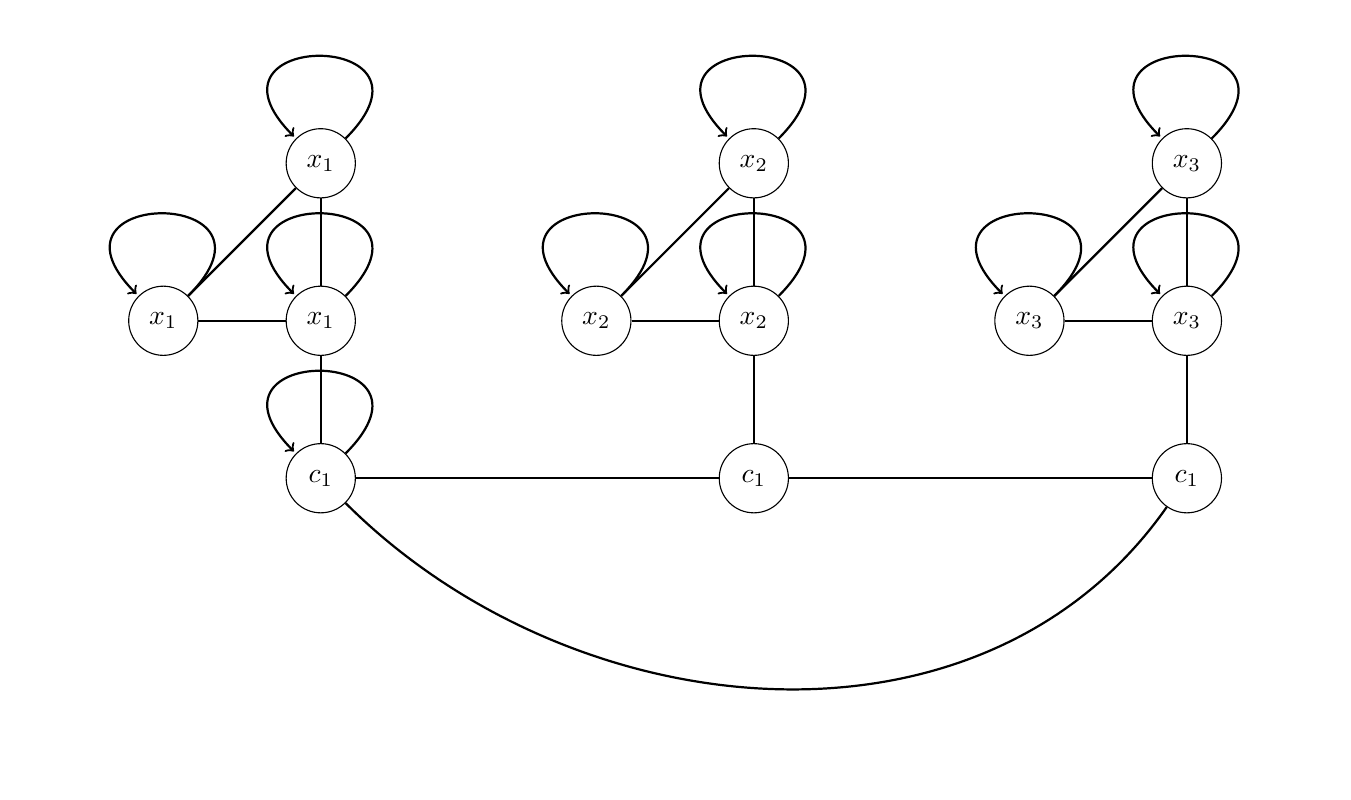
\begin{tikzpicture}[every state/.style={draw,circle},node distance=3em, inner sep=0.1cm]
\node[state] (v1) {$x_1$};
\node[state] (v2) at (-2,-2) {$x_1$};
\node[state] (v3) at (0,-2) {$x_1$};
%\node[state] (v4) at (2,-2) {$x_1$};
\node[state] (v5) at (5.5,0) {$x_2$};
\node[state] (v6) at (3.5,-2) {$x_2$};
\node[state] (v7) at (5.5,-2) {$x_2$};
%\node[state] (v8) at (7.5,-2) {$x_2$};
\node[state] (v9) at (11,0) {$x_3$};
\node[state] (v10) at (9,-2) {$x_3$};
\node[state] (v11) at (11,-2) {$x_3$};
%\node[state] (v12) at (13, -2) {$x_3$};
\node[state](v13) at (0,-4) {$c_1$};
\node[state] (v14) at (5.5, -4) {$c_1$};
\node[state] (v15) at (11, -4) {$c_1$};
\path[thick] (v1) edge (v2)
                (v2) edge (v3)
                (v6) edge (v7)
                (v10) edge (v11)
                (v3) edge (v13)
                (v7) edge (v14)
                (v11) edge (v15)
                (v13) edge [in=235, out=315] (v15)
                (v9) edge (v10)
                (v13) edge (v14)
                (v14) edge (v15)
                (v9) edge (v11)
                %(v9) edge (v12)
                (v13) edge [loop] (v13)
                (v9) edge [ loop ] (v9)
                (v10) edge [loop ] (v10)
                (v11) edge [loop ] (v11)
                %(v12) edge [loop ] (v12)
                (v5) edge (v6)
                (v5) edge (v7)
                %(v5) edge (v8)
                 (v1) edge (v3)
                 (v5) edge [loop] (v5)
                 (v6) edge [loop] (v6)
                 (v7) edge [loop] (v7)
                 %(v8) edge [loop] (v8)
                 (v2) edge [loop] (v2)
                 (v1) edge [loop] (v1)
                 (v3) edge [loop] (v3);
                 %(v4) edge [loop] (v4)
                 %(v1) edge (v4);
\end{tikzpicture}
}
\end{center}
\caption{The clause $C_1=(\bar{x}_1 \lor x_2 \lor x_3)$}
\label{fig:stable-cut}
\end{figure}
Let $H^2_1$ be the graph on $8$ vertices built from $H_1$ by subdividing all four of its pendant edges once. Call $H'$ a \emph{pendant subdivision} of $H$ if the only edges that are subdivided (perhaps many times) contain a vertex of degree $1$. Proof of the following is deferred to the appendix.

\begin{corollary}
{\sc Partially Reflexive Stable Cut} has the same classification as a C123-problem on $\mathcal{H}$-subgraph-free graphs, unless $\mathcal{H}$ contains both a pendant subdivision of a net and a pendant subdivision of $H_1$. Additionally, {\sc Partially Reflexive Stable Cut} is NP-complete on $\{C_3,H_1^2\}$-subgraph-free graphs.
\label{cor:main-stable-bis}
\end{corollary}

It follows from the previous corollary that the sets $\cal{H}$ in which the classification for {\sc Partially Reflexive Stable Cut} differs from a C123-problem must contain at least two graphs: one a pendant subdivision of a net and one pendant subdivision of $H_1$. We already saw that the $\{C_3,H_1^2\}$-subgraph-free case is NP-complete. Our further examination in this vicinity is deferred to the appendix (though the results also appear in Table~\ref{tab:1}).


\section{Surjective Homomorphism to a Cycle with a Single Loopless Vertex}\label{s-new}

To prove our next result, we rely on the problem {\sc Conflict-Free Cut}, a generalisation of {\sc Matching Cut} studied in \cite{RAUCH2025106503}. Here, an instance consists of a graph $G$ together with a graph $\hat{G}$, called a {\it conflict} graph, such that $V(\hat{G})=E(G)$. Note that two adjacent edges of $\hat{G}$ need not share any endpoints in $G$. A {\it conflict-free cut} of $G$ with respect to $\hat{G}$ is a set $F$ of edges of $G$ such that $F$ is an edge-cut of $G$ that forms an independent set of vertices in $\hat{G}$.
\begin{theorem}
\label{thm:C'r-triangle-free}
\SurHom$(C'_r)$ is NP-complete restricted to $K_3$-subgraph-free graphs for $r \geq 6$.
\end{theorem}
\begin{proof}
Let $r\geq 6$. We reduce from {\sc Conflict-Free Cut} which is NP-complete even when the conflict graph $\hat{G}$ is $1$-regular~\cite{RAUCH2025106503}, that is, even when $\hat{G}$ is an induced perfect matching. 

Given an instance $(G, \hat{G})$ of {\sc Conflict-Free Cut}, we construct an instance $G'$ of \SurHom($C'_r)$ where $C'_r$ has vertex set $\{0,1,2, \dots r-1 \}$ and $0$ is the only irreflexive vertex. We begin with an irreflexive copy of $\hat{G}$ with vertex set $M=E(G)$. Next we take a reflexive independent set $N_v= \{v'_1, \dots v'_{deg(v)}\}$, and a further reflexive vertex $v''$ which is complete to $N_v$, for each vertex $v$ of $G$. We then add an irreflexive vertex $d$ which is complete to $N=\bigcup_{v \in V(G)}N_v$. We add a reflexive pendant path on  $s=\lfloor \frac{r}{2} \rfloor-2$  vertices, $v''_{i_1} \dots v''_{i_s}$ to $v''$ for each vertex $v$ of $G$. For each edge, $e=uv$ of $G$, we choose a unique vertex $u'_i$ of $N_u$ and add the edge $eu'_i$.  We also choose a unique vertex $v'_j$ of $N_v$ and add the edge~$ev'_j$.
We refer to Figure~\ref{fig:surhom} for an illustration where $r=7$. In the same figure, we also illustrate the case $r=6$, which required us to make a slight modification of the general case, as we explain below.

We claim that $(G,\hat{G})$ has a conflict-free cut if and only if $G'$ permits a surjective homomorphism to $C'_r$.

First assume $(G, \hat{G})$ has a conflict-free cut $F$, which separates the vertices of $G$ into two sides A and B. We obtain a surjective homomorphism $h$ from $G'$ to $C'_r$ as follows. Let $h(d)=0$.
For every $i$ and $v\in A$, let $h(v'_i)=1$.
For every $i$ and $v\in B$, let $h(v'_i)=r-1$.

We now consider the (isolated) edges $ef$ in $\hat{G}$, so 
$e$ and $f$ are edges in $G$. 
As $F$ is a conflict-free cut of $(G,\hat{G})$, it holds that at most one of $e,f$ belongs to $F$.
Say $e\in F$, so $f\notin F$. We can safely set $h(e)=0$ and $h(f)=1$ or $h(f)=r-1$, depending on whether the two end-points of $f$ belong to $A$ or $B$, respectively.
Now suppose neither $e$ nor $f$ belongs to $F$.
If both $e$ and $f$ have their two endpoints both in $A$, or both in $B$, then we let
$h(e)=h(f)=1$, or $h(e)=h(f)=r-1$, respectively.
If one of them, say $e$, has its two endpoints in $A$, while $f$ has its two endpoints in $B$, then we can safely set $h(e)=1$ and $h(f)=0$.
Finally, beginning with $v''$, we map the pendant paths either to $2-3- \dots - \lfloor {\frac{r}{2}} \rfloor$ (if $h(v'_i)=1$) or $(r-2)-(r-3)- \dots -(r- \lfloor{\frac{r}{2} \rfloor})$ (if $h(v'_i)=r-1)$. This ensures the surjectivity of $h$. 

Now assume that $G'$ has a surjective homomorphism $h$ to $C'_r$. We first claim that $h(d)=0$. Assume otherwise. Since every irreflexive vertex shares a neighbour with $d$,  we may assume without loss of generality that $h(d) \in \{1,2 \}.$ For $r \geq 7$, this contradicts the surjectivity of $h$ since $d$ is joined to every other vertex of $G'$ by a path of length at most $\lfloor \frac{r}{2} \rfloor$ on which every internal vertex is reflexive.

As mentioned, for $r=6$, we slightly modify the construction by identifying the degree $1$ endpoints of each pendant path in $G'$ (which is a vertex), to a single vertex $x$. Note that we still obtain a surjective homomorphism from a conflict-free cut of $(G, \hat{G})$ as described above, since each of these identified vertices is mapped to $3$.  Now, we argue that $G'$ has diameter at most $4$. Any two vertices at a distance of at most $2$ from $d$ are at a distance of at most $4$. The only vertex $x$ with $dist(d,x)>2$ is the vertex obtained by identifying the endpoints of the reflexive paths. In this case $dist(x,v')=2$ for every $v' \in N(d)$. Hence $dist(x,y) \leq3$ for every vertex $y$ of $G'$. Now we may assume that $G'$ has no surjective homomorphism to $P'_6$, a path of length $6$ where every vertex except for one endpoint is irreflexive. In particular, this implies that, in any surjective homomorphism from $G'$ to $C_6'$, there exists a vertex  $v \in h^{-1}(0)$ which has neighbours in both $h^{-1}(1)$ and $h^{-1}(5)$. If $h(d) \in \{1,2\}$ then, since every neighbour of $d$ is reflexive, there is no vertex $y \in N^2(d)$ with $h(y)=5$. This contradicts the fact that $h$ is a surjective homomorphism, as the neighbourhood of any vertex $z \in h^{-1}(0)$ is contained in~$N^2(d)$. 
We conclude that $h(d)=0$ both if $r=6$ and $r\geq 7$.

Therefore, since $h(d)=0$ for any surjective homomorphism $h$ from $G'$ to $C'_r$, $h(v'_i) \in \{1, r-1 \}$ for each vertex $v'_i$ of $N$. We obtain a conflict-free cut of $G$ consisting of all the edges $xy$ such that $h(x'_1)\neq h(y'_1)$. By surjectivity of $h$ and the fact that each vertex $u$ of $G'$ is joined to $d$ by a path of length at most $\lfloor {\frac{r}{2}} \rfloor$ with only reflexive internal vertices, at least one vertex of $N$ is mapped to each of $1$ and $r-1$. Therefore both $A= \{v: h(v'_1)=1\}$ and $B= \{v: h(v'_1)=r-1 \}$ are non-empty. Any two vertices  $v'_i$,  $v'_j \in N(d)$ corresponding to the same vertex $v$ of $G$ are mapped to the same vertex since they share a reflexive neighbour and a neighbour $d \in h^{-1}(0)$. Therefore, if an edge has endpoints in both $A$ and $B$, its corresponding vertex in $M$ has neighbours mapped to both $r-1$ and $1$. Hence, this vertex must map to $0$. Then the set of edges with one endpoint in $A$ and the other in $B$ is contained in $h^{-1}(0)$. In particular, it induces an independent set and thus is a conflict-free cut of~$(G,\hat{G})$. 

We claim that $G'$ is $K_3$-subgraph-free. Since $N$ is an independent set, neither $d$ nor any reflexive neighbour of $v'_{i}$ is contained in a triangle. Similarly, no pendant path vertex is contained in any triangle. Then any triangle contains two adjacent vertices of $M$.  These two vertices do not share a neighbour in $M$ since $\hat{G}$ is $1$-regular. They do not share a neighbour in $N$ since each vertex of $N$ has at most one neighbour in $M$. Therefore $G'$ is triangle-free.
\end{proof}   
\begin{figure}[h]
\tikzset{every loop/.style={min distance=10mm,in=0,out=90,looseness=5}}
\begin{center} 
\resizebox{12cm}{!}{
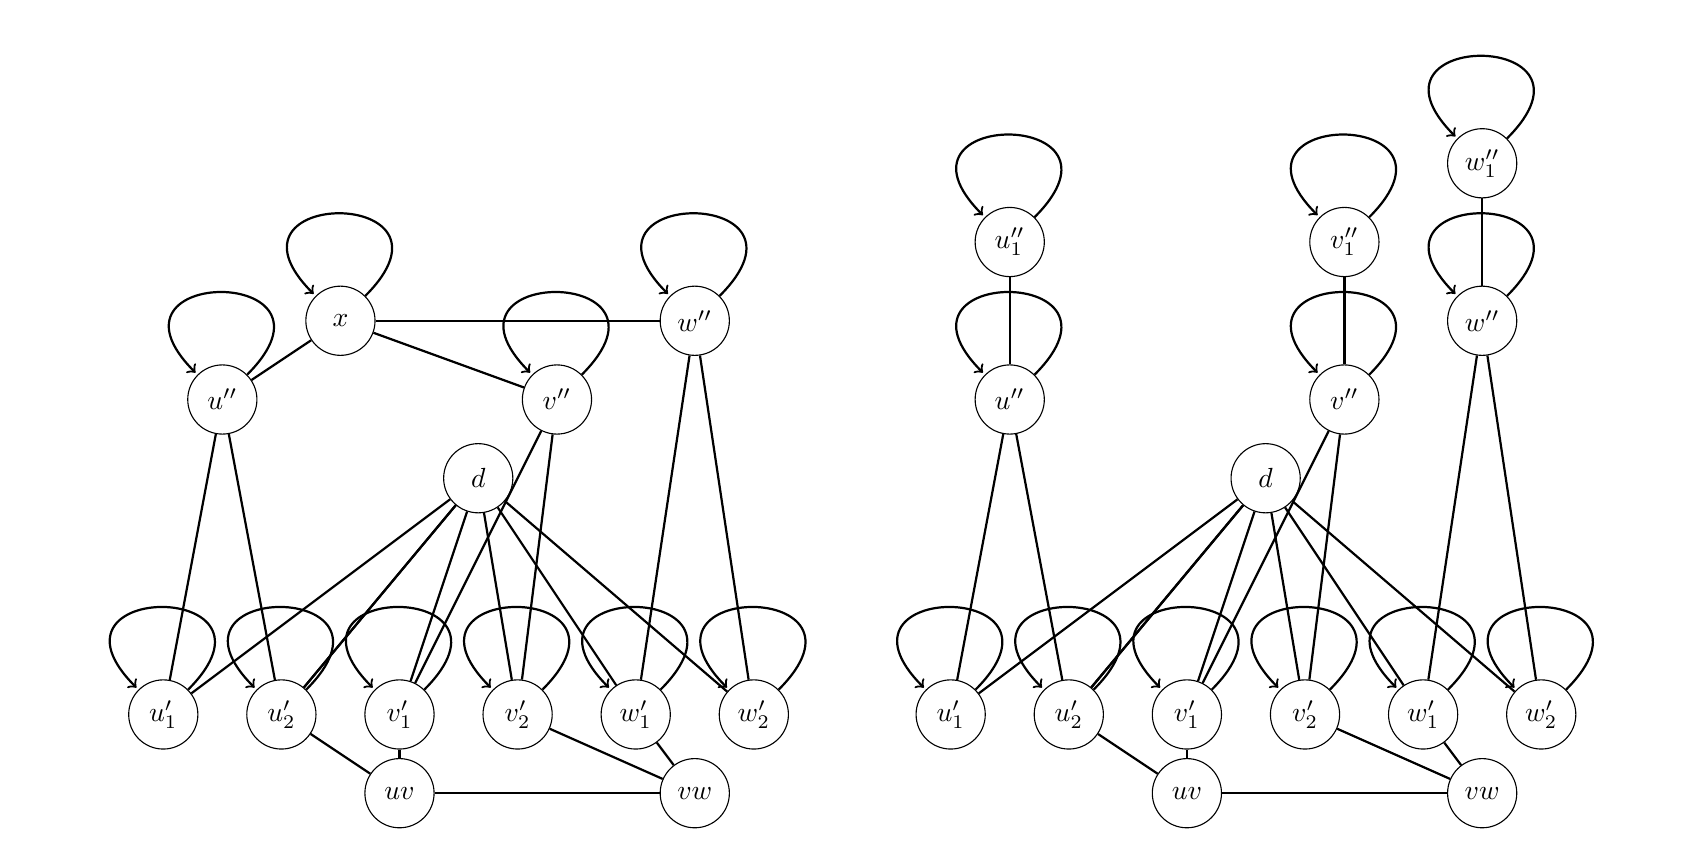
\begin{tikzpicture}[every state/.style={draw,circle},node distance=3em, inner sep=0.1cm]
\node[state] (v1) {$d$};
\node[state] (v2) at (-4,-3) {$u'_1$};
\node[state] (v3) at (-2.5,-3) {$u'_2$};
\node[state] (v4) at (-1,-3) {$v'_1$};
\node[state] (v5) at (0.5,-3) {$v'_2$};
\node[state] (v10) at (2,-3) {$w'_1$};
\node[state] (v11) at (3.5, -3) {$w'_2$};
\node[state] (v12) at (2.75,2) {$w''$};
\node[state] (v13) at (2.75, -4) {$vw$};
\node[state] (v6) at (-3.25,1) {$u''$};
\node[state] (v7) at (1,1) {$v''$};
\node[state] (v8) at (-1.75,2) {$x$};
\node[state] (v9) at (-1,-4) {$uv$};


\path[thick] (v1) edge (v2)
                (v1) edge (v10)
                (v1) edge (v11)
                (v12) edge (v10)
                (v12) edge (v11)
                (v12) edge (v8)
                (v13) edge (v5)
                (v13) edge (v10)
                (v9) edge (v3)
                (v9) edge (v4)
                (v8) edge (v6)
                (v8) edge (v7)
                (v1) edge (v3)
                (v1) edge (v4)
                (v1) edge (v5)
                (v6) edge (v3)
                (v6) edge (v2)
                (v7) edge (v5)
                (v7) edge (v4)
                (v12) edge [loop ] (v12)
                (v10) edge [loop] (v10)
                (v11) edge [loop] (v11)
                %(v5) edge (v8)
                (v13) edge (v9)
                 (v1) edge (v3)
                 (v8) edge[loop] (v8)
                 (v4) edge[loop](v4)
                 (v5) edge [loop] (v5)
                 (v6) edge [loop] (v6)
                 (v7) edge [loop] (v7)
                 %(v8) edge [loop] (v8)
                 (v2) edge [loop] (v2)
                 (v3) edge [loop] (v3);
                 %(v4) edge [loop] (v4)
                 %(v1) edge (v4);

                 \node[state] (v21) at (10,0) {$d$};
\node[state] (v22) at (6,-3) {$u'_1$};
\node[state] (v23) at (7.5,-3) {$u'_2$};
\node[state] (v24) at (9,-3) {$v'_1$};
\node[state] (v25) at (10.5,-3) {$v'_2$};
\node[state] (v210) at (12,-3) {$w'_1$};
\node[state] (v211) at (13.5, -3) {$w'_2$};
\node[state] (v212) at (12.75,2) {$w''$};
\node[state] (v213) at (12.75, -4) {$vw$};
\node[state] (v26) at (6.75,1) {$u''$};
\node[state] (v27) at (11,1) {$v''$};
\node[state] (v29) at (9,-4) {$uv$};
\node[state] (v30) at (6.75,3) {$u''_1$};
\node[state] (v31) at (11,3) {$v''_1$};
\node[state] (v32) at (12.75,4) {$w''_1$};

\path[thick] (v21) edge (v22)
            (v30) edge [loop] (v30)
            (v31)  edge [loop]  (v31)
            (v32) edge [loop] (v32)
                (v21) edge (v210)
                (v21) edge (v211)
                (v212) edge (v210)
                (v212) edge (v211)
                (v212) edge (v32)
                (v213) edge (v25)
                (v213) edge (v210)
                (v29) edge (v23)
                (v29) edge (v24)
                (v30) edge (v26)
                (v31) edge (v27)
                (v21) edge (v23)
                (v21) edge (v24)
                (v21) edge (v25)
                (v26) edge (v23)
                (v26) edge (v22)
                (v27) edge (v25)
                (v27) edge (v24)
                (v212) edge [loop ] (v212)
                (v210) edge [loop] (v210)
                (v211) edge [loop] (v211)
                %(v5) edge (v8)
                (v213) edge (v29)
                 (v21) edge (v23)
                 (v24) edge[loop](v24)
                 (v25) edge [loop] (v25)
                 (v26) edge [loop] (v26)
                 (v27) edge [loop] (v27)
                 %(v8) edge [loop] (v8)
                 (v22) edge [loop] (v22)
                 (v23) edge [loop,] (v23);
\end{tikzpicture}
}
\end{center}
\caption{The Part of $G'$ representing an edge $uv-vw$ in $\hat{G}$ in the cases $r=6$ (left) and $r=7$ (right).}
\label{fig:surhom}
\end{figure}
\begin{lemma}
    \SurHom$(C'_r)$ is trivial on graphs with diameter at least $2r-1$.
\end{lemma}
\begin{proof}
    If the input is fully reflexive then it is a no-instance. We claim all other instances are yes-instances. Let $d$ be a loopless vertex of the input $G$. Let us consider the vertex sets $V_i$ with distance $i$ from $d$. Since the diameter of $G$ is at least $2r-1$, each of $V_1,\ldots,V_{r-1}$ is non-empty. Consider the map which sends $d$ to $0$, $V_i$ to $i$ (for $i\leq r-1$) and $V_i$ to $r-1$ (for $i\geq r$). This is plainly a surjective homomorphism from $G$ to $P'_r$ (a path on $r$ vertices in which only one end vertex is loopless) and consequently to $C'_r$.
\end{proof}

\begin{corollary}
    \SurHom$(C'_r)$ is in P on all classes of bounded-degree.
    \label{cor:C'r-in-P}
\end{corollary}
\begin{proof}
    If a graph class has degree bound by $r$, then all but at most $1+c^{2r-1}$ number of graphs in that class have diameter greater than $2r-1$. We can brute force the solution to the graphs with diameter at most $2r-1$, while applying the algorithm from the previous lemma to the others.
\end{proof}
Theorem~\ref{t-4} follows directly from Theorem~\ref{thm:C'r-triangle-free} and Corollary~\ref{cor:C'r-in-P}.

\section{Final Remarks}\label{s-con}

We have shown that the C123-framework can be leveraged on enriched graph problems involving multi-edges and loops. We have shown that {\sc Multigraph Matching Cut} and {\sc Multigraph $d$-Cut} have the same classification as C123-problems.

However, our results concerning {\sc Partially Reflexive Stable Cut} are the most interesting. Owing to Corollary~\ref{cor:main-stable-bis}, we can see that {\sc Partially Reflexive Stable Cut} behaves like a C123-problem on ${\cal H}$-subgraph-free graphs unless ${\cal H}$ contains both some pendant subdivision of the net and some pendant subdivision of $H_1$. Thus, the differing behaviour comes from precisely such graphs. We have investigated this phenomenon more closely, and the third point of Corollary~\ref{cor:main-stable-bis} and Theorem~\ref{thm:tala-H2221} truly isolates the boundary of tractability, since $H^{2,2,2,1}_1$ is one vertex away from $H^2_1$. One outstanding question concerns whether {\sc Partially Reflexive Stable Cut} is in P on $\{C_3,H^{k,k,k,1}_1\}$-subgraph-free graphs, for all $k>1$.
We leave the complexity of $\SurHom(C'_5)$ tantalisingly open, in the same state as both $\SurHom(C^*_5)$ and $\SurHom(C^*_6)$.

%\bibliographystyle{acm}
\bibliography{local}

\section*{Appendix}

\subsection{Proof of Corollary~\ref{cor:main-stable-bis}.}

\


\noindent \textbf{Corollary~\ref{cor:main-stable-bis}}
{\sc Partially Reflexive Stable Cut} has the same classification as a C123-problem on $\mathcal{H}$-subgraph-free graphs, unless $\mathcal{H}$ contains both a pendant subdivision of a net and a pendant subdivision of $H_1$. Additionally, {\sc Partially Reflexive Stable Cut} is NP-complete on $\{C_3,H_1^2\}$-subgraph-free graphs.

\begin{proof}
Let us give an argument that {\sc Partially Reflexive Stable Cut} in in P on graph classes of bounded treewidth. We claim it can expressed by an $\textrm{MSO}$ formula, whereupon we may appeal to Courcelle's Theorem \cite{Courcelle}. For example, if $I$ is a new variable holding on some set of vertices, then $\forall x,y \ (I(x) \wedge I(y)) \rightarrow \neg E(x,y)$ 
    expresses that $I$ is an independent set, while
    \[
    \exists U \exists x, y \ U(x) \wedge \neg U(y) \wedge \forall x, y \ (U(x) \wedge \neg U(y) \wedge \neg I(x) \wedge \neg I(y)) \rightarrow \neg E(x,y)    
    \]
    (where $U$ is a new unary relation symbol) expresses that $E$ minus $I$ is disconnected.

If $\cal{H}$ contains any (disjoint union of) subdivisions of a path or a claw then the result clearly holds. Let us assume it does not.

If $\cal{H}$ contains a a pendant subdivision of $H_1$, but not a pendant subdivision of a net, then we may use the proof from the first part of Theorem~\ref{thm:siani-main}, taking care that our paths are long enough to omit any of the $H_1, H_2, H_3, \ldots, C_4, C_5, \ldots$ in ${\cal H}$.

If $\cal{H}$ contains only a pendant subdivision of the net, but no pendant subdivision of $H_1$, then we may use the proof from the second part of Theorem~\ref{thm:siani-main}. This construction is triangle-free so plainly omits any pendant subdivision of the net, though we need to ensure that our paths are long enough to omit any of the $H_2, H_3, \ldots, (C_3,) C_4, C_5, \ldots$ in ${\cal H}$.

For the $\{C_3,H_1^2\}$-subgraph-free case, let us return to the graph we had that was $\{C_4,C_5,\ldots,C_k,H_1,H_2,\ldots,H_k\}$-subgraph-free in the first case of Theorem~\ref{thm:siani-main}. It had many $C_3$s with one looped vertex. The idea is to subdivide only once, replacing these with $C_4$s, similarly to what we did in the proof of the second part of Theorem~\ref{thm:siani-main} (see Figure~\ref{fig:stable-C4} for guidance). The resulting graph omits both $C_3$ and $H_1^2$ as a subgraph.%\qed
\end{proof}

\begin{figure}[h]
\begin{center}
$
   \xymatrix{
& \bigcirc  \ar@{-}[d]  & \\
& \bigcirc \ar@{-}[dl] \ar@{-}[dr] & \\
\bullet \ar@{-}[rr] \ar@{-}[d]   & & \bullet \ar@{-}[d] \\
\bigcirc & & \bigcirc \\
}
$
\hspace{2cm}
$
  \xymatrix{
\bigcirc  \ar@{-}[d]  & \\
\bigcirc \ar@{-}[d] \ar@{-}[rr] & & \bigcirc \ar@{-}[d] \\
\bullet \ar@{-}[rr] \ar@{-}[d]   & & \bullet \ar@{-}[d] \\
\bigcirc & & \bigcirc \\
}
$
\end{center}
\caption{The substitution of the $C_3$s (left) by $C_4$s (right) in the proof of Corollary~\ref{cor:main-stable-bis}. Note that open circles represent looped vertices.}
\label{fig:stable-C4}
\end{figure}


\subsection{Further observations on Partially Reflexive Stable Cut}

\begin{lemma}\label{lem:gen-obs}
There exists a polynomial time algorithm which, given an instance $G$ of {\sc Partially Reflexive Stable Cut}, either finds that $G$ is a yes-instance or returns an equivalent instance $G'$ with the following properties:
\begin{itemize}
    \item[1.] Every vertex of degree $2$ is reflexive and no vertex has degree ($0$ or) $1$.
    \item[2.] No degree $2$ vertex is contained in a triangle.
    \item[3.] There are no twin vertices.
    \item[4.] For any pair $u,v \in V$, if $N(u) \subseteq N(v)$, then $u$ must be reflexive and $v$ must not be.
\end{itemize}

Moreover, any simple graph contained as a subgraph in $G'$ is contained in $G$.

\end{lemma}
\begin{proof}
{\textbf {Property 1}}:
If a vertex $v$ of $G$ has degree ($0$ or) $1$ then either $N(v)$ is a stable cut of $G$ has a stable cut if and only if $G \setminus \{v\}$ does. Therefore, we either find that $G$ is a yes-instance or obtain an equivalent instance by deleting $v$.

Let $v$ be an irreflexive degree $2$ vertex. If $v$ is a cut vertex or $N(v)$ forms a stable cutset then $G$ is a yes-instance. Else, $G$ has a stable cutset if and only if $G \setminus {v}$ does and we may delete $v$ to obtain an equivalent instance. Repeating this process exhaustively, we either find that $G$ is a yes-instance or obtain an instance in which every vertex has degree at least $2$ and every degree $2$ vertex is reflexive.

\textbf{Property 2}:
Consider a degree $2$ vertex $v$ contained in a triangle. This vertex is reflexive by Property 1. Since the neighbourhood of $v$ is a clique, $N(v)$ is not a stable cut. Since $v$ is reflexive, it does not belong to any stable cut of $G$. Therefore, any stable cut of $G$ is a stable cut of $G \setminus v$. Since exactly one side of any stable cut in $G \setminus v$ contains a neighbour of $v$, $G$ has a stable cut if and only if $G \setminus v$ does and we may delete $v$. Repeating this process exhaustively, we obtain an instance in which every degree $2$ vertex has two independent neighbours.

\textbf{Property 3}:
Assume that $G$ contains a vertex $x$ with a true twin $y$. From Property $2$ we may assume $x$ has degree at least $3$. Assume that $G$ has a stable cut $C$ containing at least one of $x$ and $y$. It contains at most one of $x$ and $y$ since they are adjacent. Without loss of generality, $C$ contains $x$. Furthermore, since $x$ and $y$ have the same open neighboburhood, removing $x$ from $C$ does not connect the graph $G \setminus {C}$. Therefore, neither $x$ nor $y$ are contained in a minimal stable cut of $G$. Therefore, $G$ has a stable cut if and only if $G \setminus \{y \}$ has a stable cut which does not contain $x$. In other words, We obtain an equivalent instance by deleting $y$ and making $x$ reflexive.

We now assume that $x$ and $y$ are false twins. If there exists a stable cut of $G$ containing exactly one, say $x$, of $x$ and $y$ then, since $x$ and $y$ have the same open neighbourhood, there exists a stable cut containing neither of them. Therefore, any minimal stable cut $C$ either contains both $x$ and $y$ or neither of the two. In particular, if either of $x$ and $y$ is reflexive then we may make the other reflexive. Now, $G$ has a stable cut if and only if $G \setminus \{x \}$ does. In other words, we obtain an equivalent instance by deleting $x$.

Repeating these steps exhaustively, we obtain a graph with no twin vertices.

\textbf{Property 4}:
Note that $u$ and $v$ are non-adjacent since $v \notin N(v)$. Assume that $u$ is irreflexive. If $N(u)$ forms a stable cut then $G$ is a yes-instance, Since every neighbour of $u$ is a neighbour of $v$, $u$ is not a cut vertex. Therefore, any stable cut of $G$ is a stable cut of $G \setminus u $. On the other hand, consider a stable cut $C$ of $G \setminus u$. If $v$ belongs to $C$ then, since $u$ is irreflexive, we may add $u$ to $C$ to obtain a stable cut of $G$. If $v$ does not belong to $C$ then we add $u$ to the same side as $v$ to obtain a stable cut of $G$. Therefore, if $u$ is irreflexive then $G$ has a stable cut if and only if $G \setminus \{u\}$ does and we may delete $u$ to obtain an equivalent instance.

Now assume that both $u$ and $v$ are reflexive. Since every neighbour of $u$ is a neighbour of $v$, $G$ has a stable cut if and only if $G \setminus u$ does and we may delete $u$ to obtain an equivalent instance.

Finally, since each of these properties is obtained through vertex deletion, any simple subgraph contained in $G'$ is contained in $G$.%\qed
\end{proof}

The next lemma deals with three additional properties which apply specifically to $H_1$-subgraph-free instances.

\begin{lemma}\label{lem:H-obs}
There exists a polynomial time algorithm which, given any $H_1$-subgraph-free instance $G$ of {\sc Partially Reflexive Stable Cut}, either decides $G$ or returns an equivalent instance $G'$ with the following properties:
\begin{enumerate}
\item[h1.] Every irreflexive vertex is contained in a triangle with another irreflexive vertex.
\item[h2.] No two triangles share a vertex.
\item[h3.] Each vertex of any triangle has exactly one neighbour outside the triangle and this vertex has degree 2.
\end{enumerate}

Moreover, any simple graph contained as a subgraph in $G'$ is contained in $G$.
\end{lemma}

\begin{proof}
We may assume that $G$ is connected and satisfies Properties 1 to 4.

\textbf{Property h1}:
Let $S$ be the set of irreflexive vertices in $G$. Note that any stable cut $C$ of $G$ is contained in $S$. By Property 1, every vertex in $S$ has degree at least $3$ in $G$. Let $v$ be a vertex in $S$ with no neighbours in $S$. Either $v$ is a cut vertex and $G$ is a yes-instance, or $G$ has a stable cut if and only if $G \setminus v$ does. Therefore we may remove any vertex which is isolated in $G[S]$ and is not a cut vertex. If this process leaves $S$ empty then $G$ is a no-instance. Otherwise, by $H_1$-subgraph-freeness, any two adjacent vertices in $S$ are contained in a triangle.

\textbf{Property h2}:
First assume that $G$ contains a diamond subgraph with vertex set $D={x,y,z,w}$ where $x$ and $y$ have degree $2$ in the diamond. Assume that $x$ and $y$ are adjacent. Then, by $H_1$-subgraph-freeness, at most one vertex outside $D$ has a neighbour in $D$. If $G=K_4$ then $G$ is a no-instance. Otherwise, either the neighbour $v$ of $D$ forms a stable cut or $G$ has a stable cut if and only if $G \setminus D$ does.

Now assume that $x$ and $y$ are non-adjacent. By Property $2$, each of them has at least one further neighbour. By $H_1$-subgraph-freeness, each of $x$ and $y$ has exactly one further neighbour. Let $a$ be a neighbour of $x$ outside $D$ and $b$ a neighbour of $y$ outside $D$. Neither $z$ nor $w$ has any neighbours outside $D \cup \{a, b \}$ by $H_1$-subgraph-freeness. If $a=b$ then $x$ and $y$ are twins, contradicting Property $3$.

Otherwise, both $a$ and $b$ have degree $2$ by $H_1$-subgraph-freeness and must be reflexive by Property $1$. Additionally, neither $z$ nor $w$ has a neighbour outside $D$ by $H_1$-subgraph-freeness. In particular, $z$ and $w$ are true twins. By Property $4$ we obtain an equivalent instance $G'$ by deleting the vertex $z$.

Now assume that the set $T \subseteq V(G)$  forms a subgraph of $G$ consisting of two triangles sharing exactly one vertex $v$. By $H_1$-subgraph-freeness and Property 1, the only vertex of $T$ which may have a neighbour outside $T$ is $v$. In particular, since we may assume that $G$ contains no diamond subgraph, the remaining vertices of $T$ have degree $2$, contradicting Property $2$.

\textbf{Property h3}:
By Property $2$ every vertex of any triangle $T$ has a neighbour outside $T$. By Property h$2$ no vertex outside $T$ has more than one neighbour in $T$. By $H_1$-subgraph-freeness each neighbour of $T$ then has degree $2$.

Finally, since each of these properties is obtained through vertex deletion, any simple subgraph contained in $G'$ is contained in $G$.%\qed
\end{proof}

\begin{lemma}
{\sc Partially Reflexive Stable Cut} is polynomial-time solvable for $\{H_1, r N_{1,1,1}\}$-subgraph-free graphs for any $r \geq 1$.
\end{lemma}

\begin{proof}
 We show that any $rN_{1,1,1}$-subgraph-free graph has at most $12r-1$ irreflexive vertices. Assume otherwise. By Properties h$2$ and h$3$, this implies that $G$ contains at least $4r$ vertex disjoint triangles. Since, by Property h$3$, any such triangle shares a neighbour with at most three others, $G$ contains at least $r$ disjoint copies of $N_{1,1,1}$, contradicting $rN_{1,1,1}$-subgraph-freeness. Therefore, we may test each possible combination of irreflexive vertices to decide whether it forms a stable cut of $G$.%\qed
\end{proof}
Together with Corollary~\ref{cor:main-stable-bis}, the previous lemma yields a proof of Theorem~\ref{t-3}. We continue however, with a view to obtaining some further results.

The following lemma is strictly incomparable to the last.
\begin{lemma}
{\sc Partially Reflexive Stable Cut} is polynomial-time solvable for $\{H_1, N_{1,1,\ell}\}$-subgraph-free graphs for any $l \geq 0$.
\end{lemma}

\begin{proof}
We may assume that $G$ contains a path $P$ of length $2\ell$ as a subgraph, else the problem is polynomial-time solvable since $P_k$-subgraph-free graphs have bounded treewidth. If every triangle in $G$ contains at least one vertex of $P$ then $G$ contains at most $2\ell$ triangles by Property h$2$ and hence at most $6\ell$ irreflexive vertices by Property h$1$. In this case we test every subset of these vertices to decide whether it forms a stable cut. Otherwise, assume $G$ contains at least $6\ell+1$ irreflexive vertices and consider a triangle $T={x,y,z}$ containing no vertex of $P$. Without loss of generality, assume that $x$ is an endpoint of a shortest path $Q$ from $T$ to $P$, intersecting $P$ at a vertex $v$. No vertex of $T$ has a neighbour on the interior of $P$ since any neighbour of $T$ has degree $2$ by Property h$3$. The vertex $v$ divides $P$ into two segments, one of which has length at least $\ell$. Therefore we may extend $Q$ to a path $Q'$ of length at least $\ell$ and obtain a subgraph $N_{1,1,\ell}$ by taking $T, Q'$ and two further neighbours of $y$ and $z$. This implies that $G$ contains at most $6\ell$ irreflexive vertices, a contradiction.%\qed 
\end{proof}

The graph $H_1^{2,2,2,1}$ is obtained by subdividing $3$ out of the $4$ pendant edges of $H_1$ (see Figure~\ref{fig:subH1}).
\begin{figure}
    \centering
    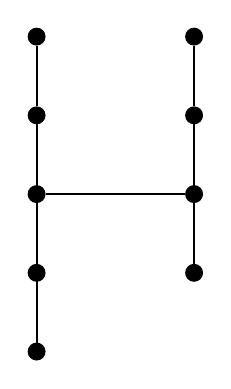
\begin{tikzpicture}[thick]
        \node[draw, circle, fill, inner sep=2pt] (A) at (0,1) {};
        \node[draw, circle, fill, inner sep=2pt] (A1) at (0,0) {};
        \node[draw, circle, fill, inner sep=2pt] (B) at (0,-2) {};
        \node[draw, circle, fill, inner sep=2pt] (B1) at (0,-3) {};
        \node[draw, circle, fill, inner sep=2pt] (C) at (2,1) {};
        \node[draw, circle, fill, inner sep=2pt] (C1) at (2,0) {};
        \node[draw, circle, fill, inner sep=2pt] (D) at (2,-2) {};
        \node[draw, circle, fill, inner sep=2pt] (E) at (0,-1) {};
        \node[draw, circle, fill, inner sep=2pt] (F) at (2,-1) {};
        
        \draw (A) -- (A1) -- (B1) -- (B);
        \draw (C) -- (C1) -- (D);
        \draw (E) -- (F);
    \end{tikzpicture}
    \caption{ $H_1^{2,2,2,1}$}
    \label{fig:subH1}
\end{figure}
We now work towards a proof of the result on the penultimate line in Table~\ref{tab:1}. The proof relies on showing that, given some $\{H_1^{2,2,2,1}, C_3\}$-subgraph-free graph after applying Lemmas~\ref{lem:gen-obs} and \ref{lem:small-cut}, the set of irreflexive vertices, $S$, forms a stable set. This implies $G$ admits a (partially reflexive) stable cut if, and only if $S$ is a cutset.

\begin{lemma}\label{lem:small-cut}
For any constant $k$, any instance of {\sc Partially Reflexive Stable Cut} can be reduced in polynomial time to an equivalent instance $G'$ such that for every $Z \subseteq V(G')$ with $\vert Z \vert \leq k$, if $G'[Z]$ is connected with maximum degree at least $3$, then $Z$ contains at least three vertices with some neighbour in $V(G')\setminus Z$.
\end{lemma}
\begin{proof}
For each $Z \subseteq V$ such that $3 \leq \vert Z \vert \leq k$ and $G[Z]$ is connected with maximum degree $\geq 3$. If $Z$ meets one of the following conditions, we either return that $G$ is a yes-instance or find some $G'$, with size less than $G$ such that $G'$ has a partially reflexive stable cut if, and only if $G$ does. Further, every simple subgraph of $G'$ is contained in $G$.

\begin{itemize}
        \item[\textbf{s1.}] If $Z$ contains some partially reflexive stable cut for $G$ return yes.
        \item[\textbf{s2.}] If there is some $v \in Z$ such that every path between $Z$ and $G \setminus Z$ contains $v$. We call this a gateway vertex. From \textbf{s1.} we may assume $Z$ does not contain some partially reflexive stable cut meaning $v$ must be reflexive. Further, no vertex of $Z$ is contained in some minimal stable cut. Let $G' =G \setminus (Z \setminus v)$.
        \item[\textbf{s3.}] If there is some pair $v,v' \in Z$ such that every path between $Z$ and $G \setminus Z$ contains either $v$ or $v'$. We call these a gateway vertices. We again may assume $Z$ does not contain some stable cut. Let $P$ be the shortest path from $v$ to $v'$ in $G[Z]$.

        We first consider the case where there is some stable set $C \subseteq Z \setminus \{v,v'\}$ such that $v$ and $v'$ are disconnected in $G[Z \setminus C]$. If $v$ is irreflexive then $C \cup v$ is a stable cut, that is we may assume $v$ and symmetrically $v'$ have a self-loop. Let $w$ be the first irrefexive vertex in $P$. We obtain $G'$ by making every vertex in $P \setminus w$ reflexive and removing vertices $Z \setminus P$.

        If there is no such set $C$, we consider the following cases: both $v,v'$ are reflexive, one is reflexive or both are irreflexive. In the first case as $v,v'$ must be in one partition of any stable cut meaning we may obtain $G'$ by making every vertex in $P$ reflexive and removing vertices $Z \setminus P$. In the second case without loss say $v$ is irreflexive. As there is no stable set $C$ as described above $Z \setminus v$ must be contained in one partition of any stable cut. We now obtain $G'$ by making every vertex in $P \setminus v$ reflexive and removing vertices $Z \setminus P$. Finally, if $v, v'$ are irreflexive, as $v,v'$ are not a stable cut they must be adjacent. No vertex of $Z \setminus \{v,v'\}$ is contained in some minimal stable cut so let $G' =G \setminus (Z \setminus \{v,v'\})$. Given $G[Z]$ contains at least one degree 3 vertex, in each case at least one vertex has been removed.
    \end{itemize}
    %\qed
\end{proof}

\begin{theorem}
{\sc Partially Reflexive Stable Cut} is polynomial-time solvable for $\{H_1^{2,2,2,1}, C_3\}$-subgraph-free graphs.
\label{thm:tala-H2221}
\end{theorem}
\begin{proof}
Let $G$ be some  $\{H_1^{2,2,2,1}, C_3\}$-subgraph-free graph. We first complete the following pre-processing steps outlined by Lemmas~\ref{lem:gen-obs} and \ref{lem:small-cut} with $k=10$.

We now claim $S$ is a stable set. Given $S$ contains all irreflexive vertices, $G$ has a partially reflexive stable cut if, and only if $S$ is also a cutset. Assume for contradiction there is some pair of adjacent irreflexive vertices $p,q$ from Property $1$ of Lemma~\ref{lem:gen-obs} both have degree $\geq 3$. As $G$ is $C_3$-subgraph-free, there are distinct vertices $a,b \in N(p)$ and $c,d \in N(q)$. Let $D=\{p,q,a,b,c,d\}$.

From Lemma~\ref{lem:small-cut}, there must be three vertices, $x,x',x'' \in D$ with some neighbour in $G \setminus D$. Further we may assume these are distinct neighbours in $G \setminus D$, else again there are some pair of gateway vertices. Without loss we may assume $x = a$ given $a,b,c,d$ are symmetric.

\begin{figure}
    \centering
    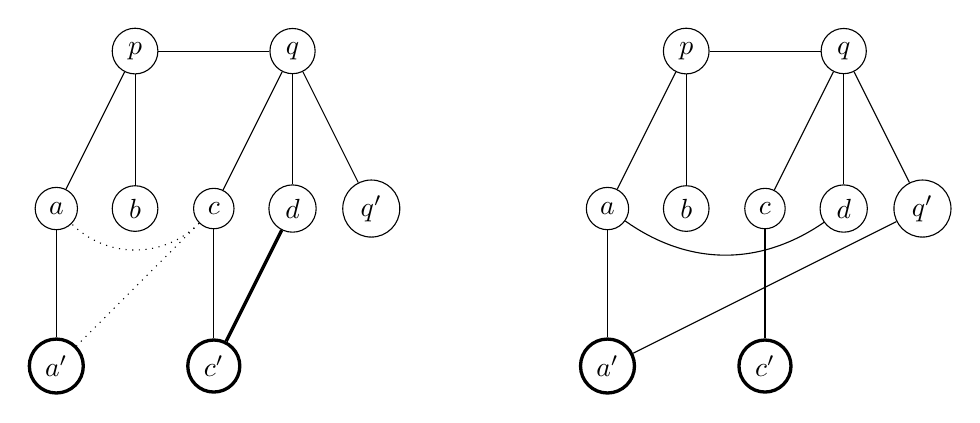
\begin{tikzpicture}[scale=1, every node/.style={circle, draw, fill=white, inner sep=3pt}]
      \node (p) at (0,2) {$p$};
      \node (q) at (2,2) {$q$};
      \node (a) at (-1,0) {$a$};
      \node[draw=black, very thick] (a') at (-1,-2) {$a'$};
      \node (b) at (0,0) {$b$};
      \node (c) at (1,0) {$c$};
      \node[draw=black, very thick] (c') at (1,-2) {$c'$};
      \node (d) at (2,0) {$d$};
      \node (q') at (3,0) {$q'$};
    
      \draw (p) -- (q);
      \draw (p) -- (a);
      \draw (p) -- (b);
      \draw (q) -- (c);
      \draw (q) -- (d);
      
      \draw (a) -- (a');
      \draw (c) -- (c');
      \draw (q) -- (q');
      \draw[very thick] (d) -- (c');
    
      \draw[bend left=45, dotted] (c) to (a);
      \draw[dotted] (c) to (a');

      \node (p2) at (7,2) {$p$};
      \node (q2) at (9,2) {$q$};
      \node (a2) at (6,0) {$a$};
      \node[draw=black, very thick] (a'2) at (6,-2) {$a'$};
      \node (b2) at (7,0) {$b$};
      \node (c2) at (8,0) {$c$};
      \node[draw=black, very thick] (c'2) at (8,-2) {$c'$};
      \node (d2) at (9,0) {$d$};
      \node (q'2) at (10,0) {$q'$};
    
      \draw (p2) -- (q2);
      \draw (p2) -- (a2);
      \draw (p2) -- (b2);
      \draw (q2) -- (c2);
      \draw (q2) -- (d2);
      
      \draw (a2) -- (a'2);
      \draw (c2) -- (c'2);
      \draw (q2) -- (q'2);
    
      \draw[bend left=35] (d2) to (a2);
      \draw (q'2) to (a'2);
    \end{tikzpicture}

\caption{\textbf{Case 1}, $x=a',x'=c'$. Left: If the edge $(d,c')$ exists, at least one of the dotted edges must exist. Right: Given $(d,c')$ is not an edge, both the edges $(a,d)$ and $(a',q')$ must exist.}
\label{fig:case1}
\end{figure}

In case 1 we assume $x'=c$, that is, there exist distinct vertices  $a' \in N(a) \setminus D$ and $c' \in N(c) \setminus D$. As $G$ is $H_1^{2,2,2,1}$-subgraph-free, $N(b) \subseteq D \cup \{a',c'\}$, symmetrically the same holds for $d$. Without loss we may assume $x'' =q$, that is there is some $q' \neq a' \neq c' \in N(q) \setminus D$. 

Further, $N(d) \subseteq \{q,a,a',c'\}$ else there is some $C_3$ or $H_1^{2,2,2,1}$ with degree 3 vertices $p,q$. Assume $d$ is adjacent to $c'$, see Figure~\ref{fig:case1} (left), now symmetrically $N(c) \subseteq \{q, a,a',c'\}$. As $N(c) \neq N(d)$ we may assume without loss $c$ is adjacent to either $a$ or $a'$. However both of these lead to a $H_1^{2,2,2,1}$ with degree $3$ vertices $c,q$. Therefore $N(d) \subseteq \{q, a,a'\}$ and symmetrically $N(q') \subseteq \{q, a,a'\}$. Both $d$ and $q'$ have degree at least $2$ and $N(d) \neq N(q')$ so without loss we may assume $a \in N(d)$ and $a' \in N(q')$, Figure~\ref{fig:case1} (right). This is a contradiction as there is some $H_1^{2,2,2,1}$ with degree 3 vertices $p,q$ concluding case 1.

\begin{figure}
    \centering
    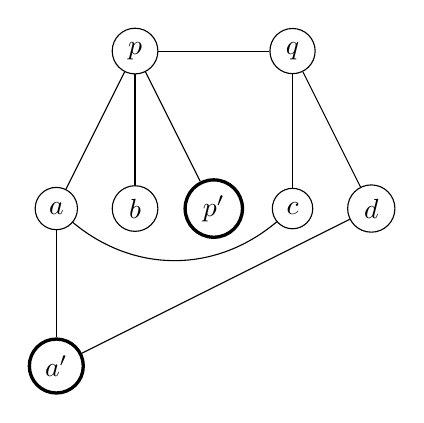
\begin{tikzpicture}[scale=1, every node/.style={circle, draw, fill=white, inner sep=3pt}]
      \node (p) at (-1,2) {$p$};
      \node (q) at (1,2) {$q$};
      \node (a) at (-2,0) {$a$};
      \node (a')[draw=black, very thick] at (-2,-2) {$a'$};
      \node (b) at (-1,0) {$b$};
      \node (c) at (1,0) {$c$};
      \node (d) at (2,0) {$d$};
      \node (p')[draw=black, very thick] at (0,0) {$p'$};
    
      \draw (p) -- (q);
      \draw (p) -- (a);
      \draw (p) -- (b);
      \draw (q) -- (c);
      \draw (q) -- (d);
      
      \draw (a) -- (a');
      \draw (p) -- (p');
    
      \draw[bend left=40] (c) to (a);
      \draw (d) to (a');
    \end{tikzpicture}
\caption{\textbf{Case 2}, $x=a',x'=p'$. The edges $(a,c)$ and $(a',d)$ must exist else this is case 1.}
\label{fig:case2}
\end{figure}

For case 2 we assume $x' = p$, that is there are distinct vertices $a' \in N(a) \setminus D$ and $p' \in N(p) \setminus D$. Now $N(c) \subseteq D \cup \{p',a'\}$ else this is case 1. Likewise $c$ is not adjacent to $p'$ (symmetrically $b$) else again this is case 1 relabelling $p'$ as $c'$. Given $G$ is $C_3$-subgraph-free, $N(c) \subseteq \{q,a,a'\}$ and symmetrically $N(d) \subseteq \{q,a,a'\}$. As both $c$ and $d$ have degree at least $2$ and $N(c) \neq N(d)$ without loss $a \in N(c)$ and $a' \in N(d)$, given $c$ and $d$ are not necessarily incomparable, we do assume $a \notin N(d)$. See Figure~\ref{fig:case2}. We now consider the possible $x''$ vertices, claiming each result in something isomorphic to case 1. If $x'' =q$, there is some $q' \neq p' \neq q' \in N(q) \setminus D$, which is case 1 given the following relabelling: $$l_1 : (p,q,a,b,c,d,a',p',q') \to (p,q,a,b,a',c,c',p',d)$$ If $x''=b$, then $b' \neq p' \neq q' \in N(b) \setminus D$, again this is case 1 given the following relabelling: $$l_2 : (p,q,a,b,c,d,a',p',b') \to (p,q,b,a,d,c,c',p',a')$$ This concludes case 2.

\begin{figure}
    \centering
    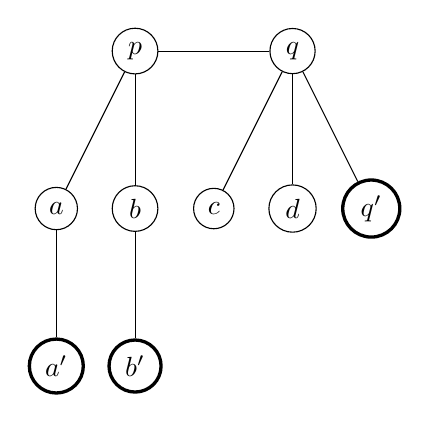
\begin{tikzpicture}[scale=1, every node/.style={circle, draw, fill=white, inner sep=3pt}]
      \node (p) at (0,2) {$p$};
      \node (q) at (2,2) {$q$};
      \node (a) at (-1,0) {$a$};
      \node (a')[draw=black, very thick] at (-1,-2) {$a'$};
      \node (b) at (0,0) {$b$};
      \node (b')[draw=black, very thick] at (0,-2) {$b'$};
      \node (c) at (1,0) {$c$};
      \node (d) at (2,0) {$d$};
      \node (q')[draw=black, very thick] at (3,0) {$q'$};
    
      \draw (p) -- (q);
      \draw (p) -- (a);
      \draw (p) -- (b);
      \draw (q) -- (c);
      \draw (q) -- (d);
      
      \draw (a) -- (a');
      \draw (b) -- (b');
      \draw (q) -- (q');
    \end{tikzpicture}
    
    \caption{\textbf{Case 3}, $x=a',x'=b', x''=q'$}
    \label{fig:case3}
\end{figure}

This leaves only case 3 where $x'=b$ and $x'' = q$, that is there are distinct vertices $a' \in N(a) \setminus D$ and $b' \in N(b) \setminus D$ and  $q' \in N(q) \setminus D$, Figure~\ref{fig:case3}. As previously $N(c) \subseteq D \cup \{a',b',q'\}$ else this is case 1. Further if $c$ is adjacent to $b'$, then relabelling $b'$ to $c'$ shows again we are in case 1. Symmetrically, $c$ is not adjacent to $a'$ and given $G$ is $C_3$-subgraph-free, $N(c) \subseteq \{q,a,b\}$. As $N(c) \subseteq N(p)$, $c$ must be reflexive. Notice $c,d,q'$ are symmetric cases so all must be reflexive and $N(\{c,d,q'\}) \subseteq \{q,a,b\}$. Given every vertex has degree at least $2$ there must be some pair $v \neq v' \in \{c,d,q'\}$ , such that $N(v) \subseteq N(v')$. However as $c,d,q'$ are each reflexive this is a contradiction. %\qed
\end{proof}
Together with Corollary~\ref{cor:main-stable-bis}, the previous theorem yields another proof of Theorem~\ref{t-3}.

\end{document}


Our proof borrows heavily from \cite{QCSPforests} which is itself based on \cite{MatchingCut} (see also \cite{GolovachPaulusmaSong} though the reduction there is not suitable for us).
\begin{figure}
\begin{center}
%\input{P101-gadgets-retraction.pdftex_t}
%
%  Created by WinFIG version 4.0 beta 1 
%  METADATA <version>1.0</version> 
%
\setlength{\unitlength}{3947sp}%
%
\begingroup\makeatletter\ifx\SetFigFont\undefined%
\gdef\SetFigFont#1#2#3#4#5{%
  \reset@font\fontsize{#1}{#2pt}%
  \fontfamily{#3}\fontseries{#4}\fontshape{#5}%
  \selectfont}%
\fi\endgroup%
\begin{picture}(5217,1776)(224,-1225)
%  METADATA <id>8</id> 
{\color[rgb]{0,0,0}\thinlines
\put(2349,346){\circle{46}}
}%
%  METADATA <id>11</id> 
{\color[rgb]{0,0,0}\put(2337,-1067){\circle{46}}
}%
%  METADATA <id>18</id> 
{\color[rgb]{0,0,0}\put(2824,-379){\circle{46}}
}%
%  METADATA <id>21</id> 
{\color[rgb]{0,0,0}\put(1887,-379){\circle{46}}
}%
%  METADATA <id>9</id> 
{\color[rgb]{0,0,0}\put(4724,370){\circle{46}}
}%
%  METADATA <id>10</id> 
{\color[rgb]{0,0,0}\put(4712,-1043){\circle{46}}
}%
%  METADATA <id>14</id> 
{\color[rgb]{0,0,0}\put(474,-330){\circle{46}}
}%
%  METADATA <id>19</id> 
{\color[rgb]{0,0,0}\put(4249,-342){\circle{46}}
}%
%  METADATA <id>20</id> 
{\color[rgb]{0,0,0}\put(5212,-342){\circle{46}}
}%
%  METADATA <id>23</id> 
{\color[rgb]{0,0,0}\put(3549, 82){\circle{46}}
}%
%  METADATA <id>24</id> 
{\color[rgb]{0,0,0}\put(3549,-793){\circle{46}}
}%
%  METADATA <id>36</id> 
{\color[rgb]{0,0,0}\put(2112,  7){\circle{46}}
}%
%  METADATA <id>38</id> 
{\color[rgb]{0,0,0}\put(2562, 20){\circle{46}}
}%
%  METADATA <id>39</id> 
{\color[rgb]{0,0,0}\put(2124,-730){\circle{46}}
}%
%  METADATA <id>40</id> 
{\color[rgb]{0,0,0}\put(2525,-730){\circle{46}}
}%
%  METADATA <id>41</id> 
{\color[rgb]{0,0,0}\put(4487, 33){\circle{46}}
}%
%  METADATA <id>42</id> 
{\color[rgb]{0,0,0}\put(4937, 45){\circle{46}}
}%
%  METADATA <id>43</id> 
{\color[rgb]{0,0,0}\put(4487,-730){\circle{46}}
}%
%  METADATA <id>44</id> 
{\color[rgb]{0,0,0}\put(4925,-742){\circle{46}}
}%
%  METADATA <id>45</id> 
{\color[rgb]{0,0,0}\put(3199,-130){\circle{46}}
}%
%  METADATA <id>46</id> 
{\color[rgb]{0,0,0}\put(3875,-117){\circle{46}}
}%
%  METADATA <id>47</id> 
{\color[rgb]{0,0,0}\put(3187,-580){\circle{46}}
}%
%  METADATA <id>48</id> 
{\color[rgb]{0,0,0}\put(3862,-580){\circle{46}}
}%
%  METADATA <id>58</id> 
{\color[rgb]{0,0,0}\put(2345,-1148){\circle{138}}
}%
%  METADATA <id>59</id> 
{\color[rgb]{0,0,0}\put(4707,-1123){\circle{138}}
}%
%  METADATA <id>60</id> 
{\color[rgb]{0,0,0}\put(5295,-336){\circle{138}}
}%
%  METADATA <id>61</id> 
{\color[rgb]{0,0,0}\put(4720,439){\circle{138}}
}%
%  METADATA <id>63</id> 
{\color[rgb]{0,0,0}\put(4332,-323){\circle{138}}
}%
%  METADATA <id>64</id> 
{\color[rgb]{0,0,0}\put(2757,-374){\circle{138}}
}%
%  METADATA <id>65</id> 
{\color[rgb]{0,0,0}\put(2357,426){\circle{138}}
}%
%  METADATA <id>66</id> 
{\color[rgb]{0,0,0}\put(1819,-374){\circle{138}}
}%
%  METADATA <id>68</id> 
{\color[rgb]{0,0,0}\put(382,-337){\circle{138}}
}%
%  METADATA <id>71</id> 
{\color[rgb]{0,0,0}\put(3544,139){\circle{138}}
}%
%  METADATA <id>72</id> 
{\color[rgb]{0,0,0}\put(3557,-874){\circle{138}}
}%
%  METADATA <id>27</id> 
{\color[rgb]{0,0,0}\put(1876,364){\line( 1, 0){3313}}
}%
%  METADATA <id>30</id> 
{\color[rgb]{0,0,0}\put(1876,-1049){\line( 1, 0){3313}}
}%
%  METADATA <id>35</id> 
{\color[rgb]{0,0,0}\put(1876,-374){\line( 2, 3){492.308}}
\put(2351,376){\line( 3,-5){447.706}}
\put(2814,-361){\line( 5, 3){740.441}}
\put(3551, 89){\line( 5,-3){682.353}}
\put(4239,-311){\line( 2, 3){463.231}}
\put(4714,376){\line( 3,-4){516}}
\put(5214,-324){\line(-3,-4){542.760}}
\put(4689,-1061){\line(-3, 5){458.735}}
\put(4226,-299){\line(-4,-3){679.680}}
\put(3539,-799){\line(-5, 3){735.882}}
\put(2801,-361){\line(-2,-3){457.692}}
\put(2326,-1036){\line(-2, 3){455.539}}
}%
%  METADATA <id>49</id> 
{\color[rgb]{0,0,0}\put(2101, 14){\line( 1, 0){438}}
}%
%  METADATA <id>50</id> 
{\color[rgb]{0,0,0}\put(2114,-724){\line( 1, 0){400}}
}%
%  METADATA <id>51</id> 
{\color[rgb]{0,0,0}\put(4476,-724){\line( 1, 0){425}}
}%
%  METADATA <id>52</id> 
{\color[rgb]{0,0,0}\put(4476, 51){\line( 1, 0){450}}
}%
%  METADATA <id>53</id> 
{\color[rgb]{0,0,0}\put(3189,-124){\line( 1, 0){675}}
}%
%  METADATA <id>54</id> 
{\color[rgb]{0,0,0}\put(3176,-574){\line( 1, 0){675}}
}%
%  METADATA <id>81</id> 
{\color[rgb]{0,0,0}\put(2112,-15){\line( 0,-1){706}}
}%
%  METADATA <id>82</id> 
{\color[rgb]{0,0,0}\put(2539, -7){\line( 0,-1){706}}
}%
%  METADATA <id>83</id> 
{\color[rgb]{0,0,0}\put(4487,  0){\line( 0,-1){706}}
}%
%  METADATA <id>84</id> 
{\color[rgb]{0,0,0}\put(4930, 24){\line( 0,-1){706}}
}%
%  METADATA <id>85</id> 
{\color[rgb]{0,0,0}\put(3175,-147){\line( 0,-1){434}}
}%
%  METADATA <id>86</id> 
{\color[rgb]{0,0,0}\put(3873,-109){\line( 0,-1){434}}
}%
%  METADATA <id>73</id> 
\put(5376,301){\makebox(0,0)[lb]{\smash{{\SetFigFont{12}{14.4}{\rmdefault}{\mddefault}{\updefault}{\color[rgb]{0,0,0}$\top$}%
}}}}
%  METADATA <id>74</id> 
\put(5376,-1111){\makebox(0,0)[lb]{\smash{{\SetFigFont{12}{14.4}{\rmdefault}{\mddefault}{\updefault}{\color[rgb]{0,0,0}$\bot$}%
}}}}
%  METADATA <id>77</id> 
\put(1564,-474){\makebox(0,0)[lb]{\smash{{\SetFigFont{12}{14.4}{\rmdefault}{\mddefault}{\updefault}{\color[rgb]{0,0,0}$l_1$}%
}}}}
%  METADATA <id>78</id> 
\put(3289,114){\makebox(0,0)[lb]{\smash{{\SetFigFont{12}{14.4}{\rmdefault}{\mddefault}{\updefault}{\color[rgb]{0,0,0}$l_2$}%
}}}}
%  METADATA <id>79</id> 
\put(5426,-411){\makebox(0,0)[lb]{\smash{{\SetFigFont{12}{14.4}{\rmdefault}{\mddefault}{\updefault}{\color[rgb]{0,0,0}$l_3$}%
}}}}
%  METADATA <id>75</id> 
\put(239,-199){\makebox(0,0)[lb]{\smash{{\SetFigFont{12}{14.4}{\rmdefault}{\mddefault}{\updefault}{\color[rgb]{0,0,0}$v_1$}%
}}}}
\end{picture}%

\end{center}
\caption{Variable and clause gadgets in reduction to $\SurHom(P_{101})$. Each of $l_1,l_2,l_3$ will have degree three when linked to their corresponding variables.}
\label{fig:sur-hom-gadgets}
\end{figure}
\begin{proposition}
\label{prop:sur-hom-P101}
$\SurHom(P_{101})$ is NP-complete.
\end{proposition}
\begin{proof}
For hardness, we reduce from (monotone) \emph{not-all-equal 3-satisfiability}, whose NP-completeness is well known \cite{Papa}. From an instance $\Phi$ of NAESAT we will build an instance $G$ of QCSP$(P_{101})$ such that $\Phi$ is NAE3SAT iff $G$ has a surjective homomorphism to $P_{101}$.

We begin by describing the graph $G=G_\Phi$. The construction of $G_\Phi$ begins with two reflexive paths, labelled $\top$ and $\bot$ which contain in between them gadgets for the clauses and variables of $\Phi$. We begin by assuming that the paths $\top$ and $\bot$ are evaluated to vertices $1$ and $3$ in $P_{101}$, respectively (the two ends of $P_{101}$); later on we will show how this is ensured by the surjectivity of the homomorphism. Of course, once one vertex of one of the paths is evaluated to, say, $1$, then that whole path must also be so evaluated -- as the only looped neighbour of $1$ in $P_{101}$ is $1$. The gadgets are drawn in Figure~\ref{fig:sur-hom-gadgets}.
%We will return to the question of the absence of vertical bracing at the end of the proof.

For each variable $v_1$ in $\Phi$ we add the gadget drawn on the left. For each clause of $\Phi$ we introduce a copy of the clause gadget drawn on the right. We then introduce an edge between a variable $v$ and literal $l_i$ ($i \in \{1,2,3\}$) if $v=l_i$ (note that all literals in monotone NAE3SAT are positive). It is not hard to verify that homomorphisms from $G_\Phi$ to $P_{101}$ (such that the paths $\top$ and $\bot$ are evaluated to $1$ and $3$, respectively) correspond exactly to satisfying not-all-equal assignments of $\Phi$. The looped vertices must map to either $1$ or $3$ -- $\top$ or $\bot$ -- and the clause gadgets forbid exactly the all-equal assignments.

In order to conclude the proof, we must argue that it is not possible, in a surjective homomorphism, for both the paths $\top$ or $\bot$ to map (w.l.o.g.) to $1$.  Indeed, suppose to the converse that both reflexive paths of $G_\Phi$ map in some homomorphism to the same end of $P_{101}$. Considering the clause gagdgets of Figure~\ref{fig:sur-hom-gadgets}, we can see that no vertex could ever map to the other end of $P_{101}$ and therefore the homomorphism could not have been surjective.
\end{proof}
Let $C'_{11}$ be the cycle on vertices $\{-5,\ldots,5\}$ all of whose vertices are looped except $0$ which is loopless. We aim to adapt the proof of the previous proposition in order to prove the following.
\begin{proposition}
\label{prop:sur-hom-Cdash9}
$\SurHom(C'_{11})$ is NP-complete.
\end{proposition}
Our principal challenge is ensuring that the paths $\top$ and $\bot$ are mapped to $-1,1$ or $1,-1$. The first thing we notice is that we can make the following amendments to the produced graph $G_\Phi$ without affecting the properties of the reduction. We begin by merging all loops on the path $\top$ to make $a$ and all loops on the path $\bot$ to make $b$. Then, for all pairs of looped vertices we add a new vertex to produce a path of length $2$ between them in the new graph $G'_\Phi$. It is plain to see that $G'_\Phi$ has diameter $4$ as all loopless vertices have a neighbour that is looped.

We finally add a reflexive path of length $4$ to $a$ and a reflexive path of length $4$ to $b$. Call the resulting instance $G''_\Phi$.

\begin{lemma}
In any surjective homomorphism from $G''_\Phi$ to $C'_{11}$, the vertices $a$ and $b$ must evaluate to $\{-3,...,3\}$.
\end{lemma}
\begin{proof}
Each of $a$ and $b$ is at distance at most 3 from any nonloop vertex and some nonloop must map to $0$.    
\end{proof}
\begin{lemma}
    Loops $a$ and $b$ must be at distance at most $2$ from one another.
\end{lemma}
\begin{proof}
    There is a path of length two between them (indeed they share an intermediate loopless vertex).
\end{proof}
\begin{lemma}
    Loops $a$ and $b$ cannot be mapped to vertices of the same sign in $C'_{11}$.
\end{lemma}
\begin{proof}
    Suppose \mbox{w.l.o.g.} both are mapped to positive integers. If they are both mapped to the same vertex $i$ or adjacent vertices $i$,$i+1$ then it should be impossible to cover the vertex $-(5-i)$. Here we are using that the cycle is long enough that $-(5-i)$ cannot be covered just using the diameter of the main gadget and the length of the reflexive paths. Thus both are mapped at distance $2$ (w.l.o.g. to $1$ and $3$). But now $-3$ cannot be covered. This is because the reflexive path whose end was evaluated as $1$ cannot cross the loopless vertex $0$, and the fact that in $G'_\phi$ all vertices are of distance at most $3$ from $a$ or $b$.
\end{proof} 
\begin{proof}[of Proposition~\ref{prop:sur-hom-Cdash9}]
We deduce from the previous three lemmas that $a,b$ map either to $1,-1$ or $-1,1$. The attached paths allow us to achieve surjectivity. The gadgets now act faithfully on the subgraph induced by $\{1,0,-1\}$ which is $P_{101}$. The argument concludes as in Proposition~\ref{prop:sur-hom-P101}. 
\end{proof}

\begin{comment}
\begin{theorem}
\SurHom($C'_r$) is NP-complete for $r \geq 6$.
\end{theorem}

\begin{proof}
We reduce from {\sc Matching Cut}. Given an instance $G$ of this problem, we construct an instance $G'$ of \SurHom($C'_r$), where $C'_r$ has vertex set $\{0,1,2, \dots r-1 \}$ and $0$ is the only irreflexive vertex. First, we take a set $M$ with one irreflexive vertex $u_e$ for each edge $e$ of $G$. We add edges so that $G'(M)$ induces $L(G)$. We then add a vertex set $N$ with one reflexive vertex v' for each vertex $v$ of $G$. We add edges $u_ea'$ and $u_eb'$ for each edge $e=ab$ of $G$. Next, we add a single irreflexive vertex $d$ which dominates $N$. Finally, we add pendant reflexive paths $P_v$ on $k=\lfloor \frac{r}{2} \rfloor-1$ vertices, $v'_1 \dots v'_{k}$ to each vertex of  $N$ and add edges so that the degree $1$ endpoints of these paths induce a clique.

We first suppose that $G$ has a matching cut $(A, B)$ with a set $C$ of cut edges. Then we obtain a surjective homomorphism $h$ from $G'$ to $C'_r$. Set $h(d)=0 $ and $ h(u_e)=0$ for $e \in C $. Then let $h(u_e)=h(a')=h(b')$ where $e=ab \notin C$, Next, $ h(v')=r-1$ for $v' \in A$ and $h(v')=1$ for $H \in B$. Finally, we set $h(v'_i)=i+1$ if $h(v')=1$ and $h(v'_i)=r-1-i$ otherwise for each vertex of each reflexive path $P_v$. $h$ is surjective since both $A$ and $B$ are non-empty by definition of a matching cut. Given two vertices $u_e$ and $u_f$, $e,f \in C$, $u_e$ is not adjacent to $u_f$ and neither of these vertices is adjacent to $d$. If $h(u_e)=1$ and $h(u_f)=r-1$ for two vertices $u_e$ and $u_f$ of $M$, then $u_e$ is an edge inside $B$ and $u_f$ is an edge inside $A$. Therefore $u_e$ and $u_f$ are non-adjacent since the two edges $e$ and $f$ do not share an endpoint. Finally, the end vertices of each pendant path either map to $\lfloor r \rfloor$ (if $r$ is even) or to one of $\lfloor \frac{r}{2} \rfloor$ and $\lfloor \frac{r}{2} \rfloor +1$ (if $r$ is odd). In either case, any two vertices of the clique evaluate to adjacent vertices on $C'_r$. Therefore $h$ is a surjective homomorphism.

Now assume that $G'$ has a surjective homomorphism $h$ to $C'_r$. We claim that $h(d)=0$. We first consider the case $r \geq 7$. Assume otherwise. Then, since every other irreflexive vertex shares a neighbour with $d$, without loss of generality we may assume $h(d) \in \{1,2\}$. Since $d$ is joined to every other vertex by a path of length at most $\lfloor \frac{r}{2} \rfloor$ whose every internal vertex is reflexive, $h(x) < 2+\lfloor \frac{r}{2} \rfloor$  for every $x \in V(G')$. This contradicts the surjectivity of $h$ since $r-1> 2+ \lfloor \frac{r}{2} \rfloor$ for $r \geq 7$. 

It remains to consider the case $r=6$. We first note that in this case the diameter of $G'$ is at most $4$ and hence $G'$ has no surjective homomorphism to $P'_6$, a path on $6$ vertices where every vertex except for one endpoint is reflexive. If $G'$ has no edge $h^{-1}(0)h^{-1}(1)$ or no edge $h^{-1}(0)h^{-1}(5)$ then $h$ is a surjective homomorphism from $G'$ to $P'_6$. Therefore we may assume that each of these edges exist. If $h(d) \in \{1,2 \}$ then $h(v')=1$ for any neighbour $v' \in N$ of a vertex in $h^{-1}(0)$. Furthermore, since any neighbour $u_f \in M$ of a vertex $u_e \in h^{-1}(0)$ shares a neighbour in $N$ with $u_e$ by definition of $L(G)$, we also have $h(u_f)=1$. This implies that $h(d)=0$.

We then obtain a matching cut of $G$ by letting $A$ be the set of vertices $v$ with $h(v')=1$ and $B$ the set of vertices $v$ with $h(v')=r-1$. Each vertex is contained in at most one cut edge since any two cut edges incident on the same vertex are adjacent in $G'(M)$ but must both belong to $h^{-1}(0)$.
\end{proof}
\end{comment}
